\documentclass[10pt,a4paper]{article}
\usepackage[margin=1.6cm]{geometry}
\usepackage{graphicx,float,hyperref,lmodern}
\usepackage[font=small,labelfont=bf]{caption}
\setlength{\parindent}{0pt}
\title{Deployment Evidence (Screenshots)\\\large Cloud Computing (SE-490) CEA --- AWS ap-south-1}
\author{Source code: \url{https://github.com/nabeedjamshedali/Axon}}
\date{}
\begin{document}
\maketitle
All screenshots were captured by browser automation from the AWS console (account Nabeed, Mumbai region) and GitHub.

\section*{Network / VPC configuration and subnets}
\begin{figure}[H]\centering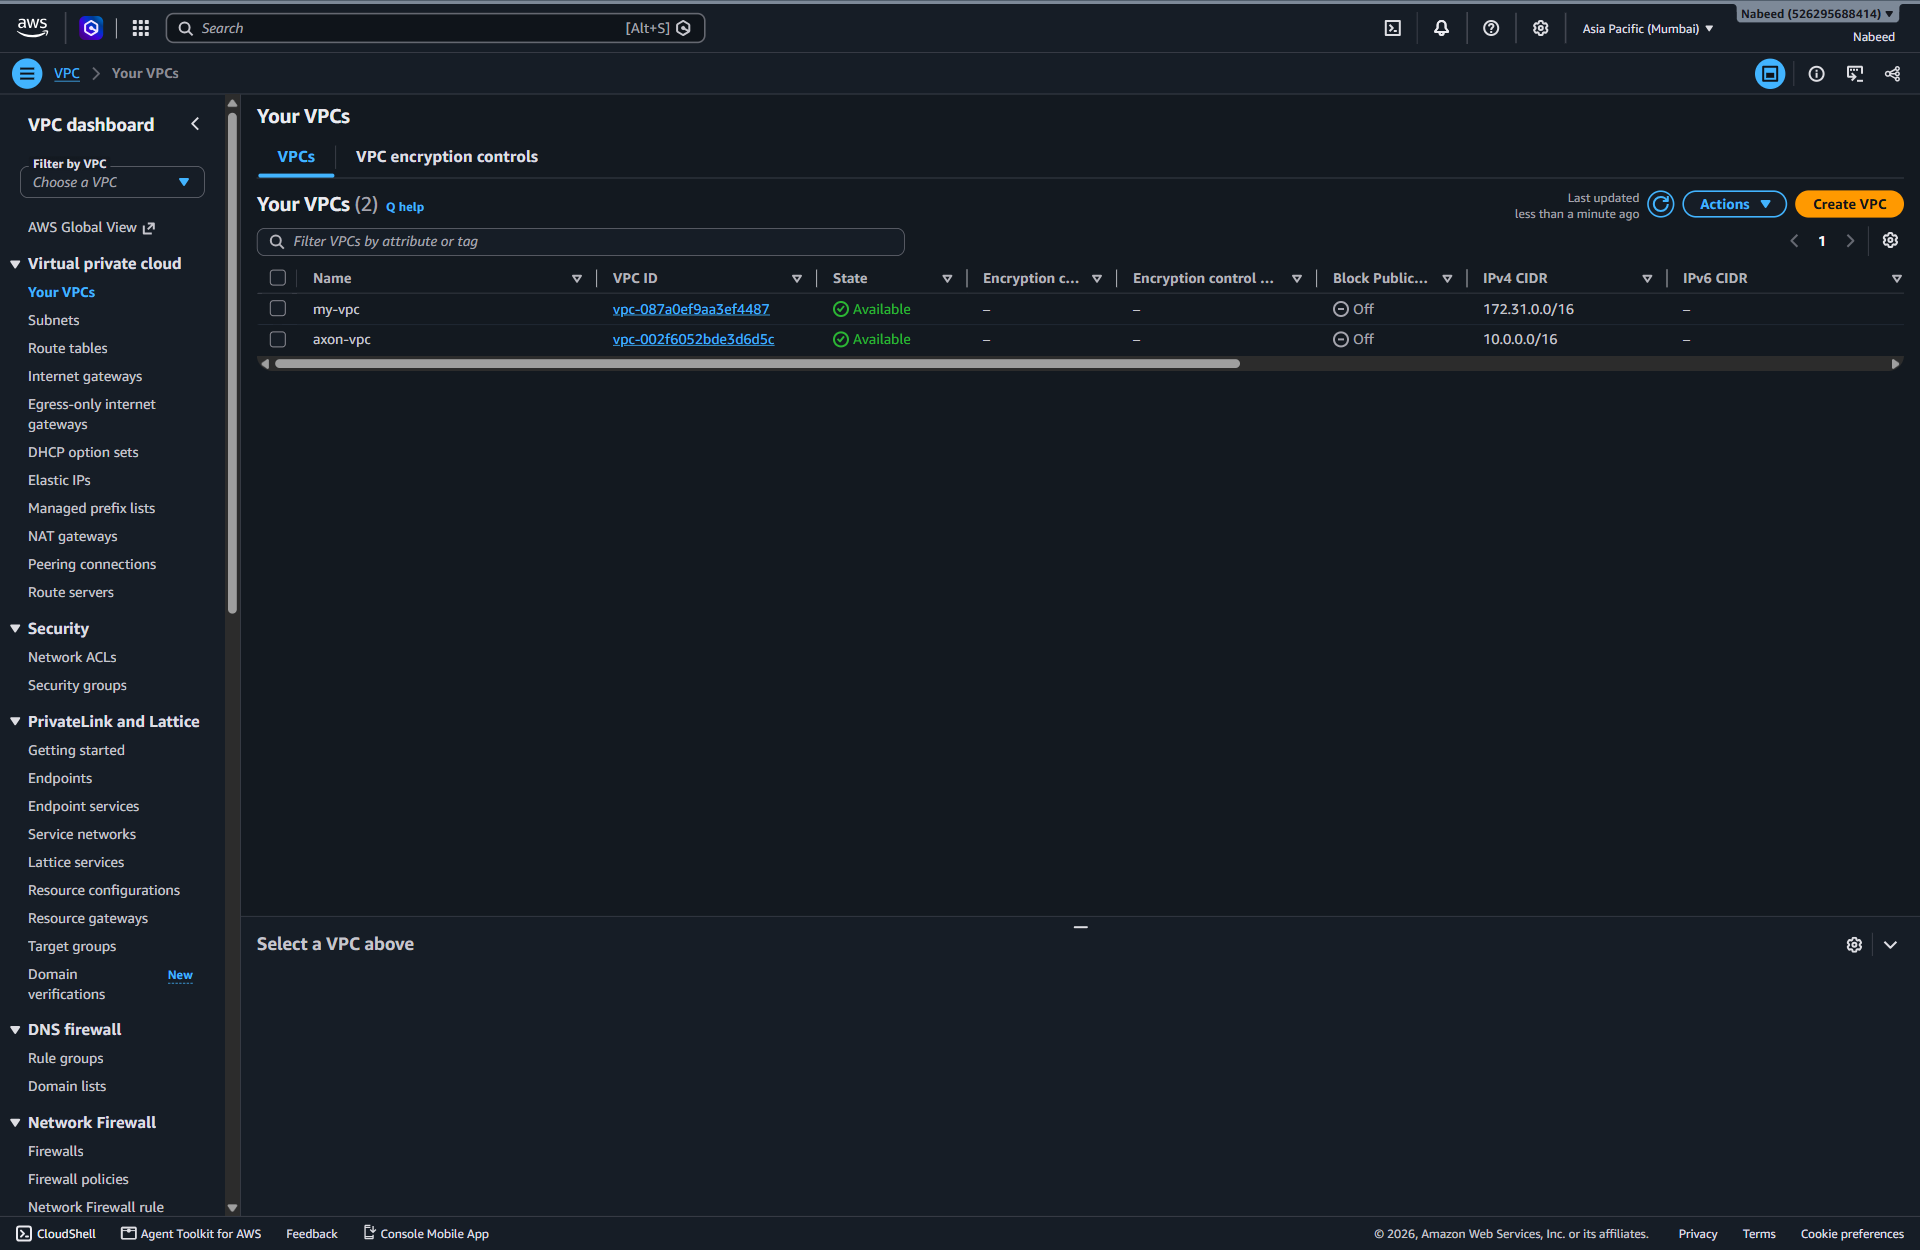
\includegraphics[width=\textwidth]{images/01-vpc.png}\caption{VPC \texttt{axon-vpc} (10.0.0.0/16) in ap-south-1.}\end{figure}
\begin{figure}[H]\centering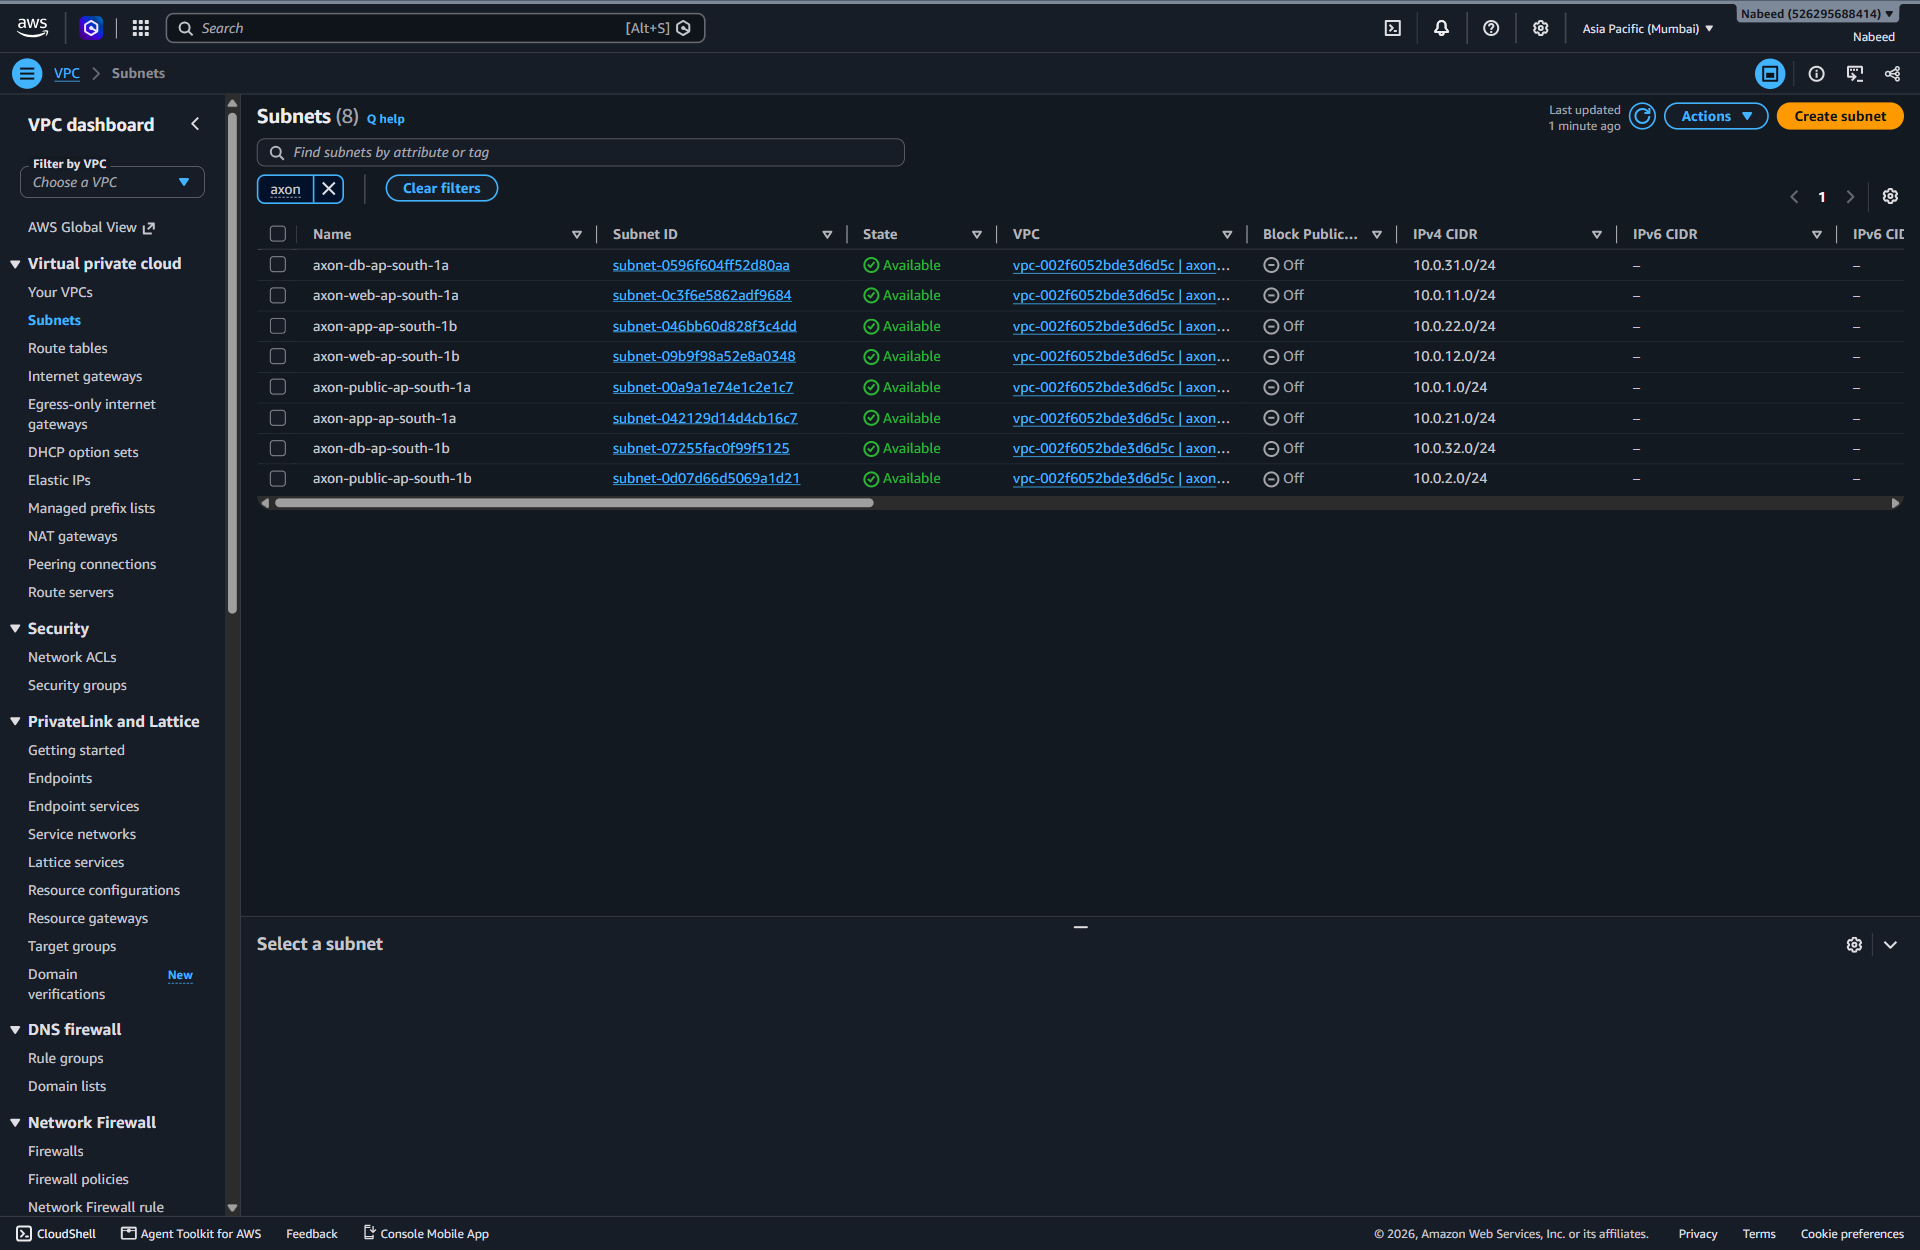
\includegraphics[width=\textwidth]{images/02-subnets.png}\caption{Eight subnets across two AZs: public, web, app and DB tiers.}\end{figure}
\begin{figure}[H]\centering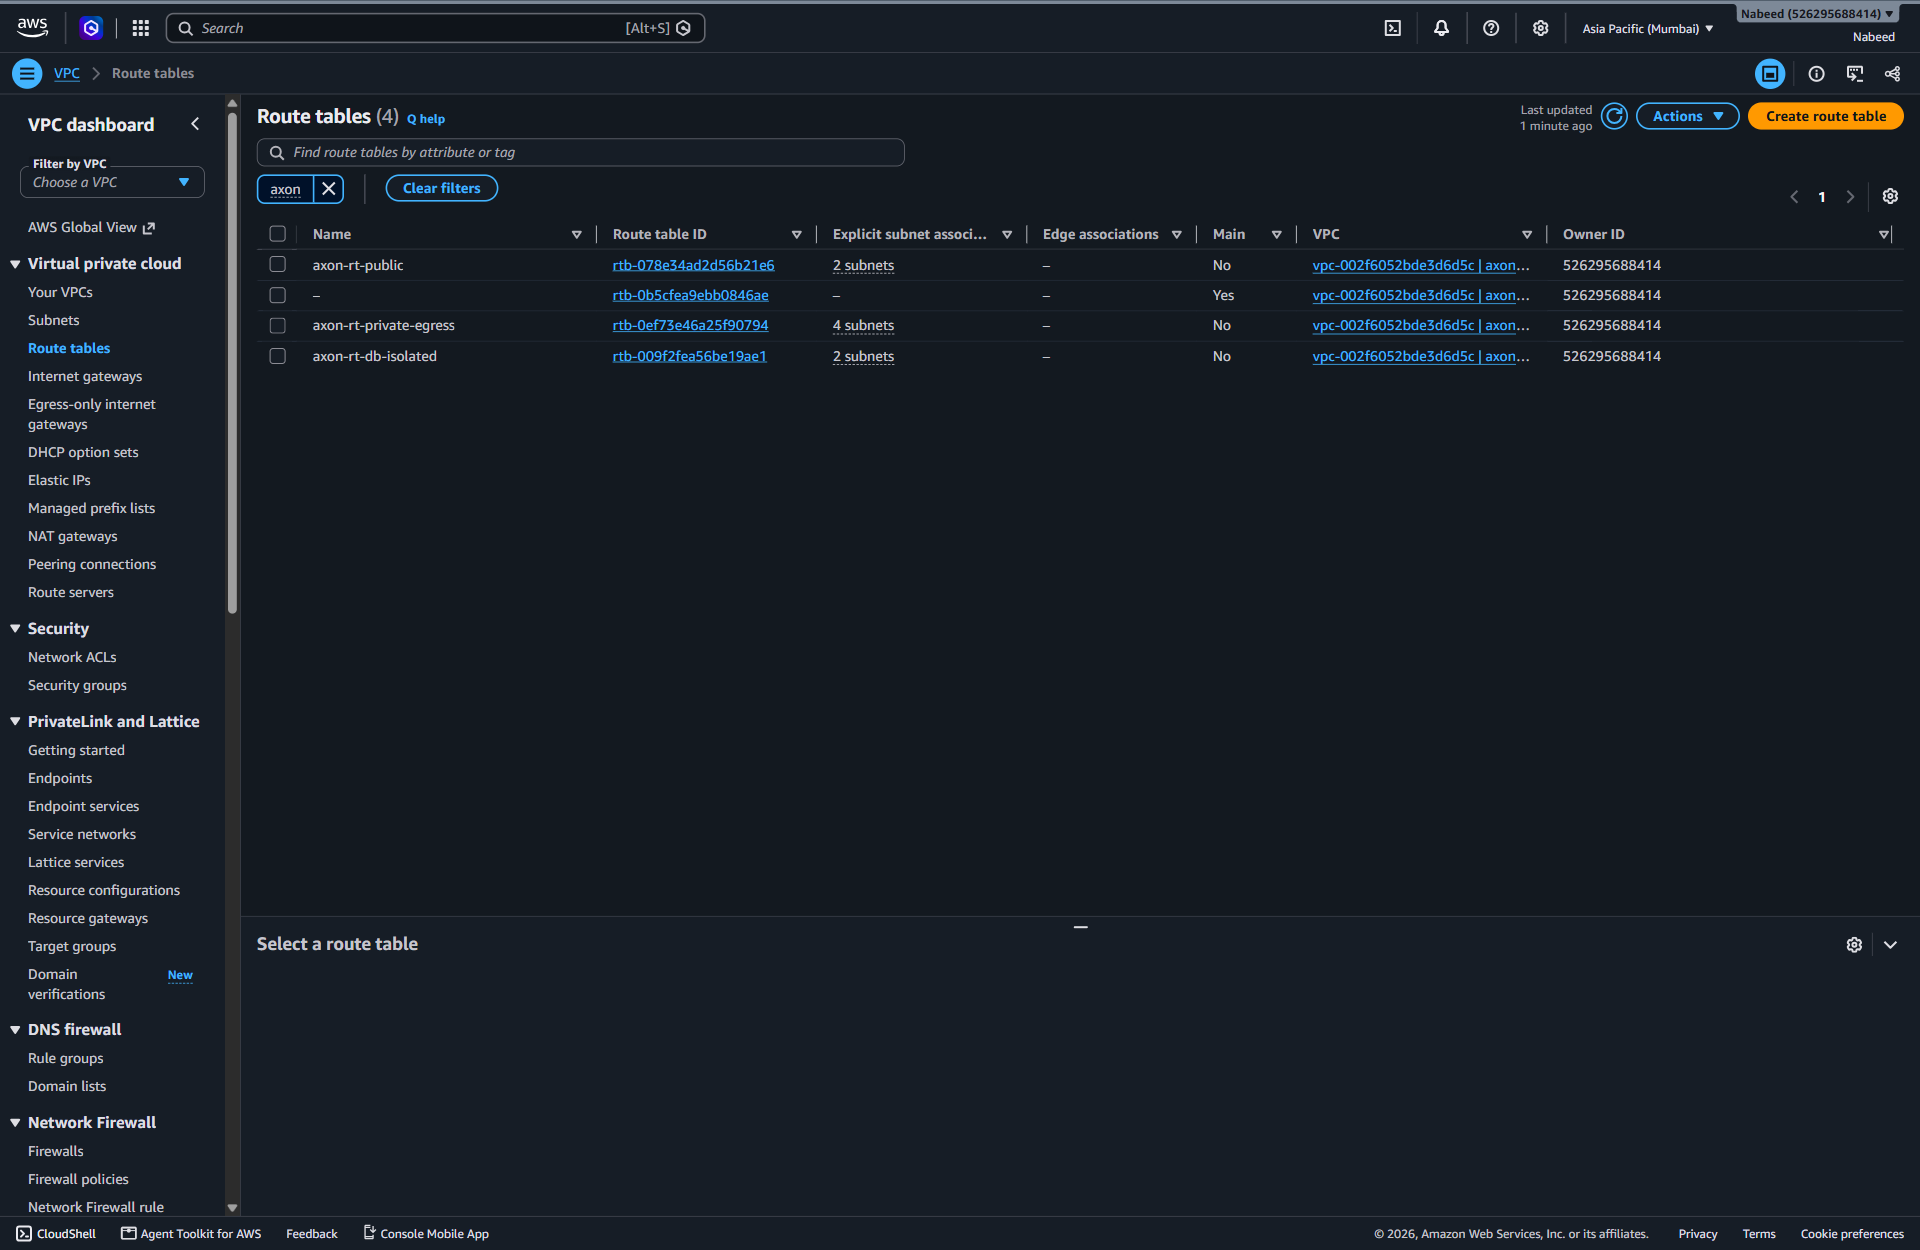
\includegraphics[width=\textwidth]{images/03-route-tables.png}\caption{Route tables: public (IGW), private egress (NAT) and isolated DB table.}\end{figure}
\begin{figure}[H]\centering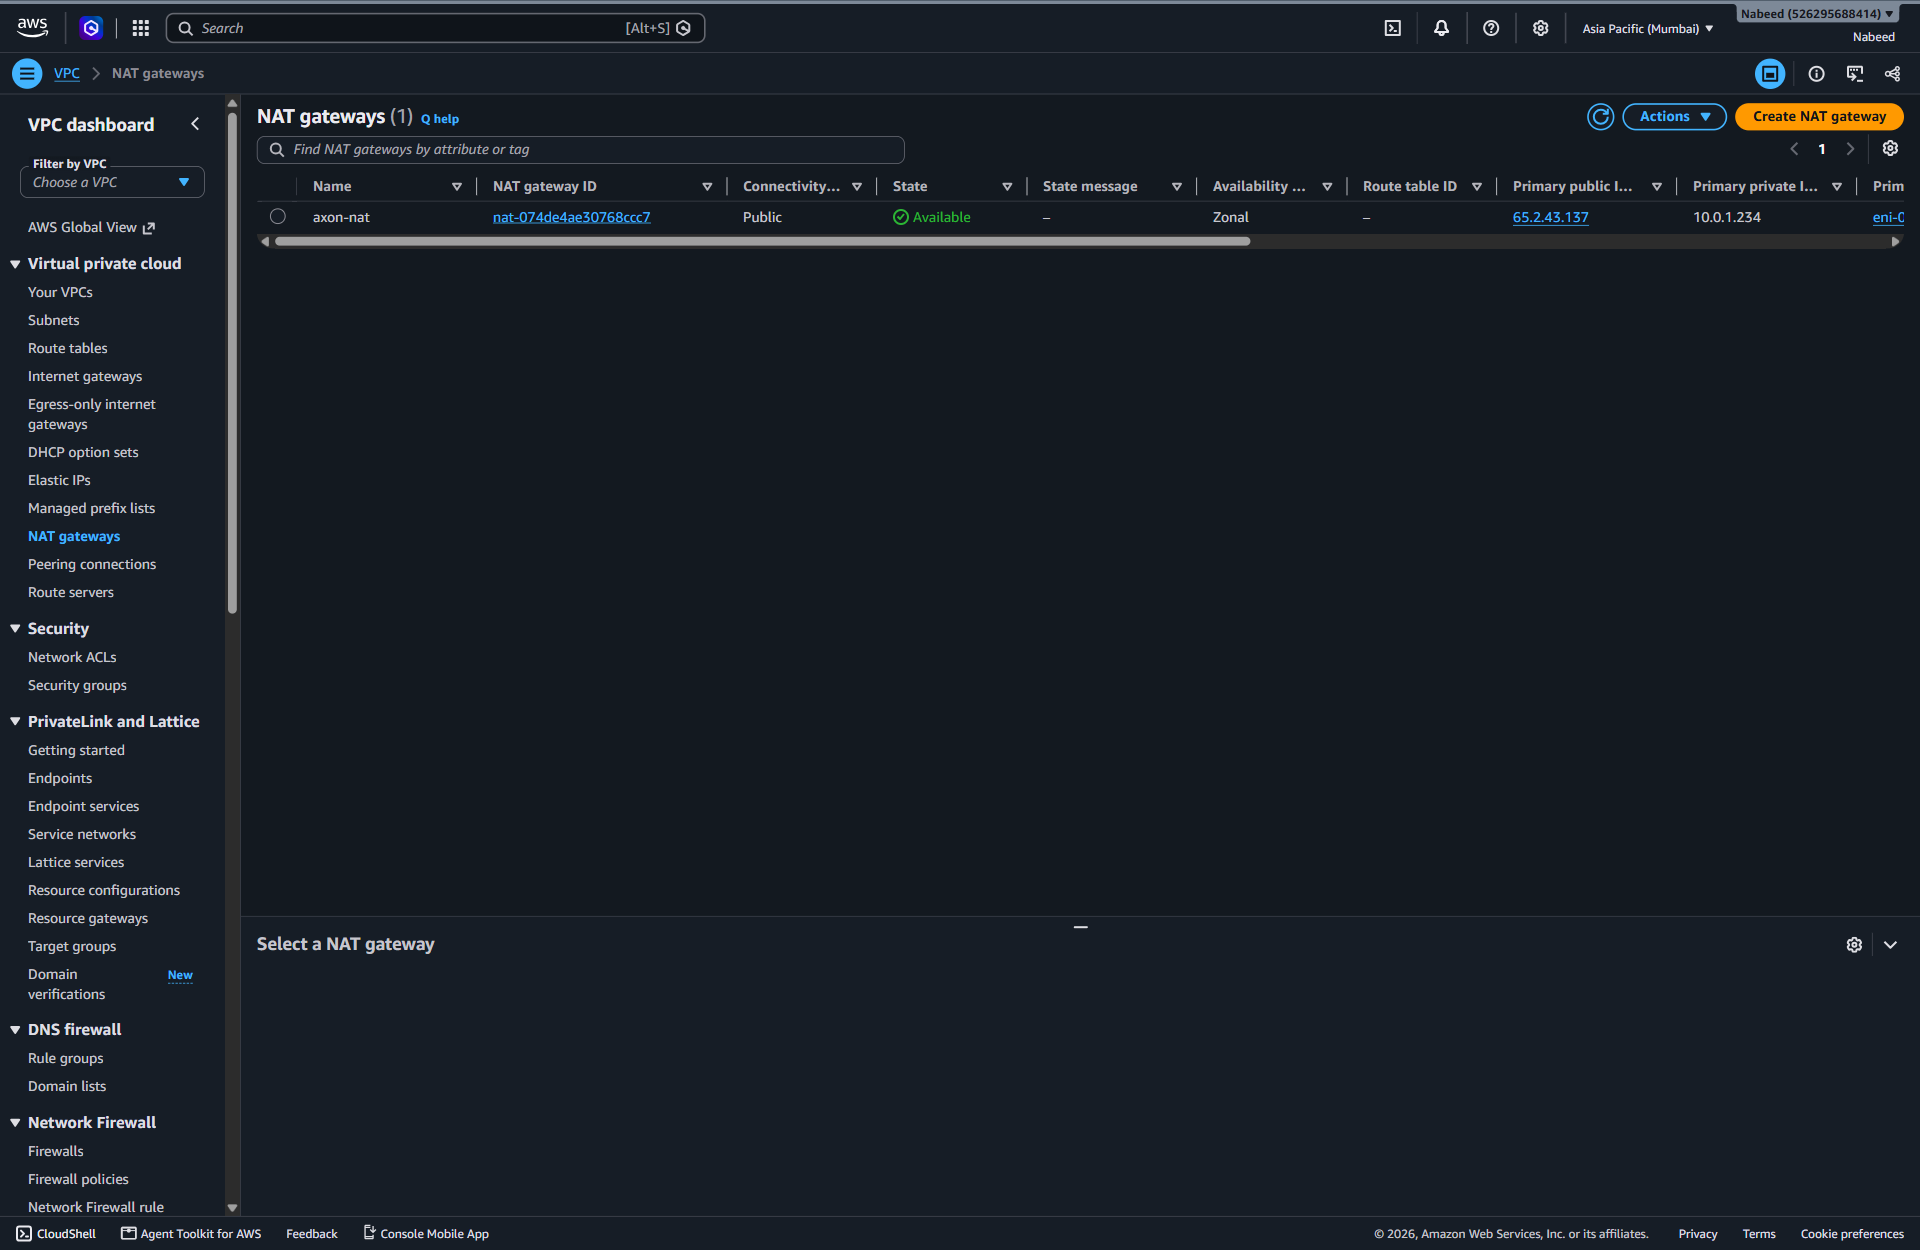
\includegraphics[width=\textwidth]{images/04-nat-gateway.png}\caption{NAT gateway in a public subnet.}\end{figure}
\section*{Compute instances / container hosts}
\begin{figure}[H]\centering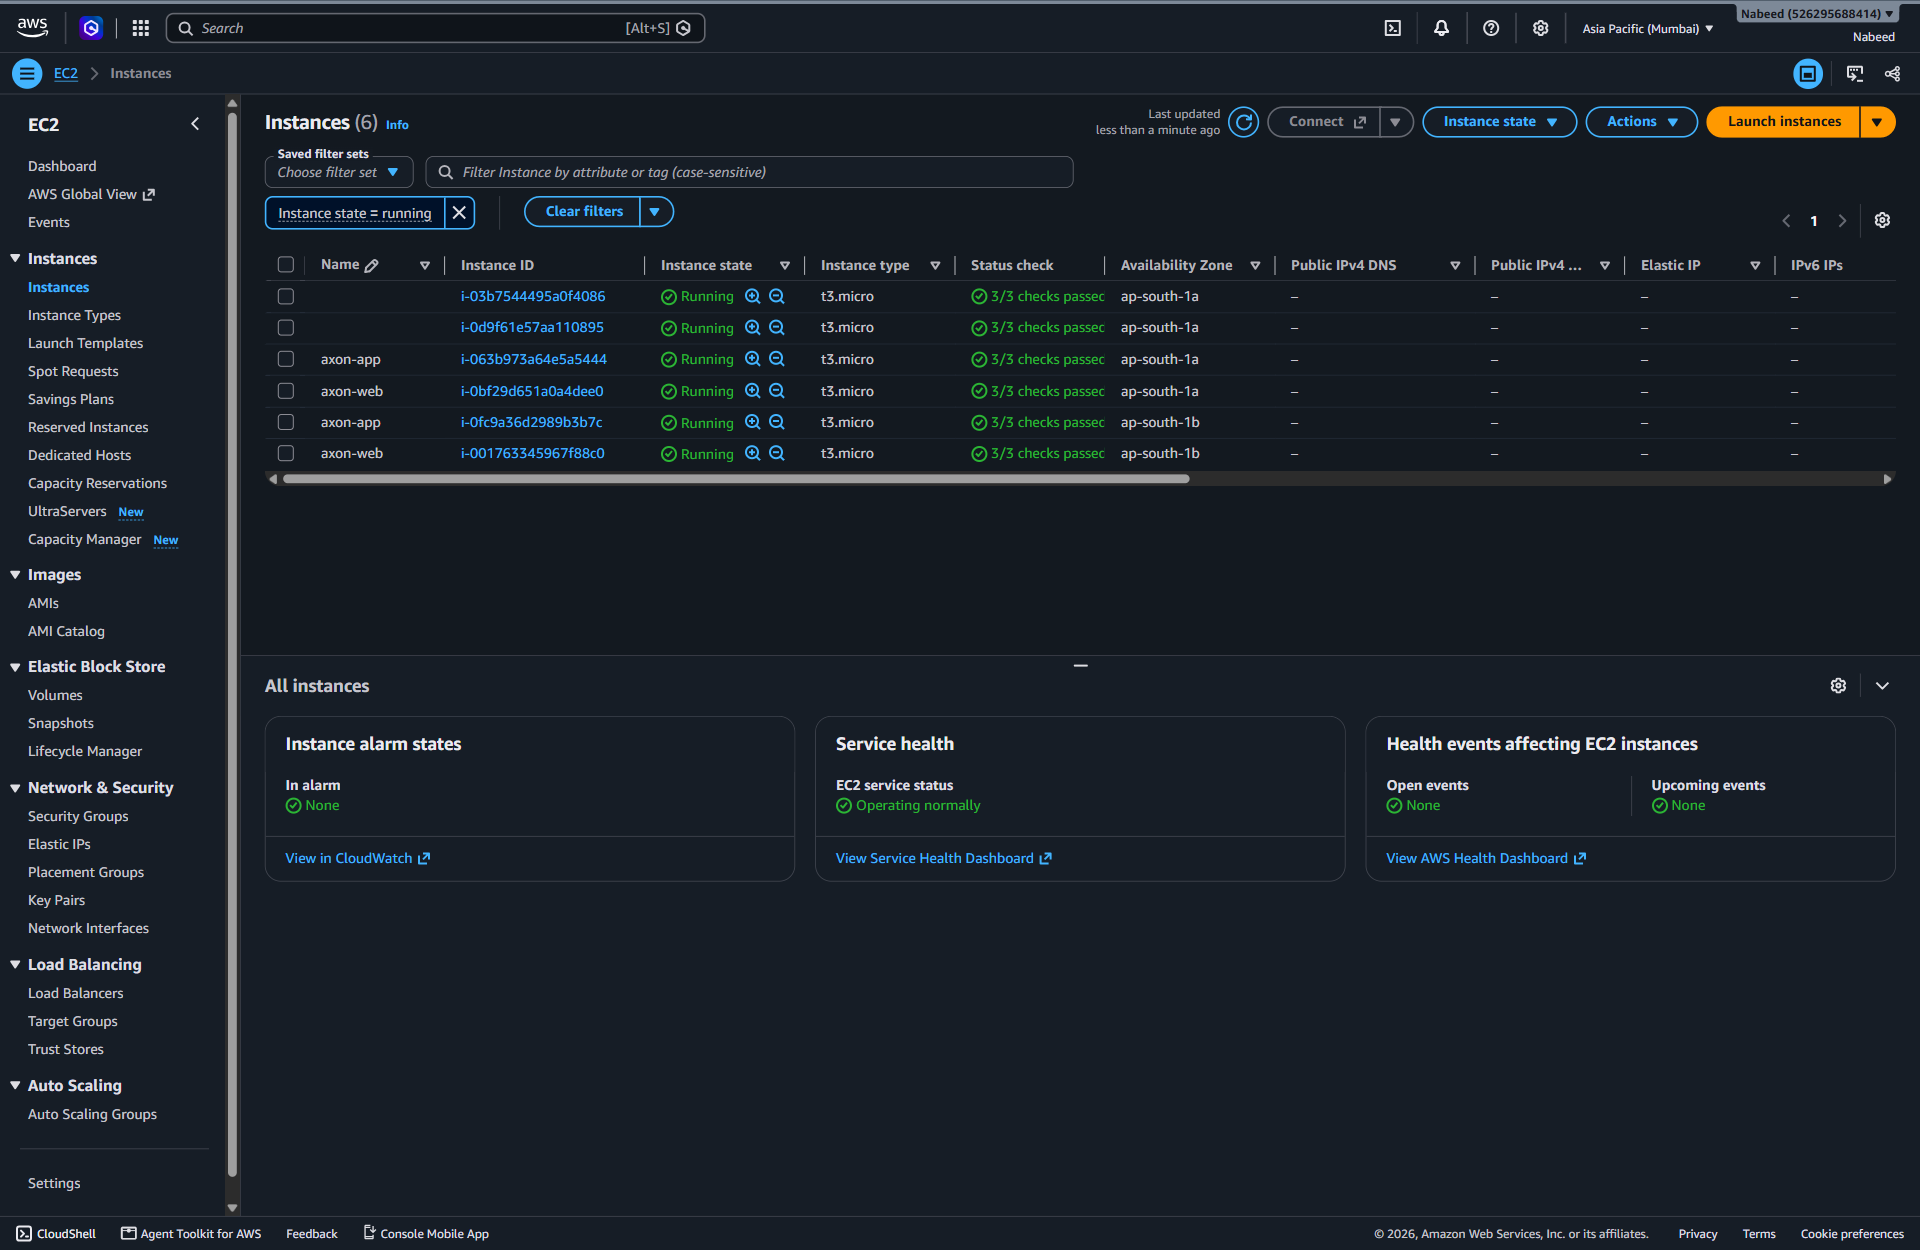
\includegraphics[width=\textwidth]{images/05-ec2-instances.png}\caption{Running web-tier and app-tier instances.}\end{figure}
\begin{figure}[H]\centering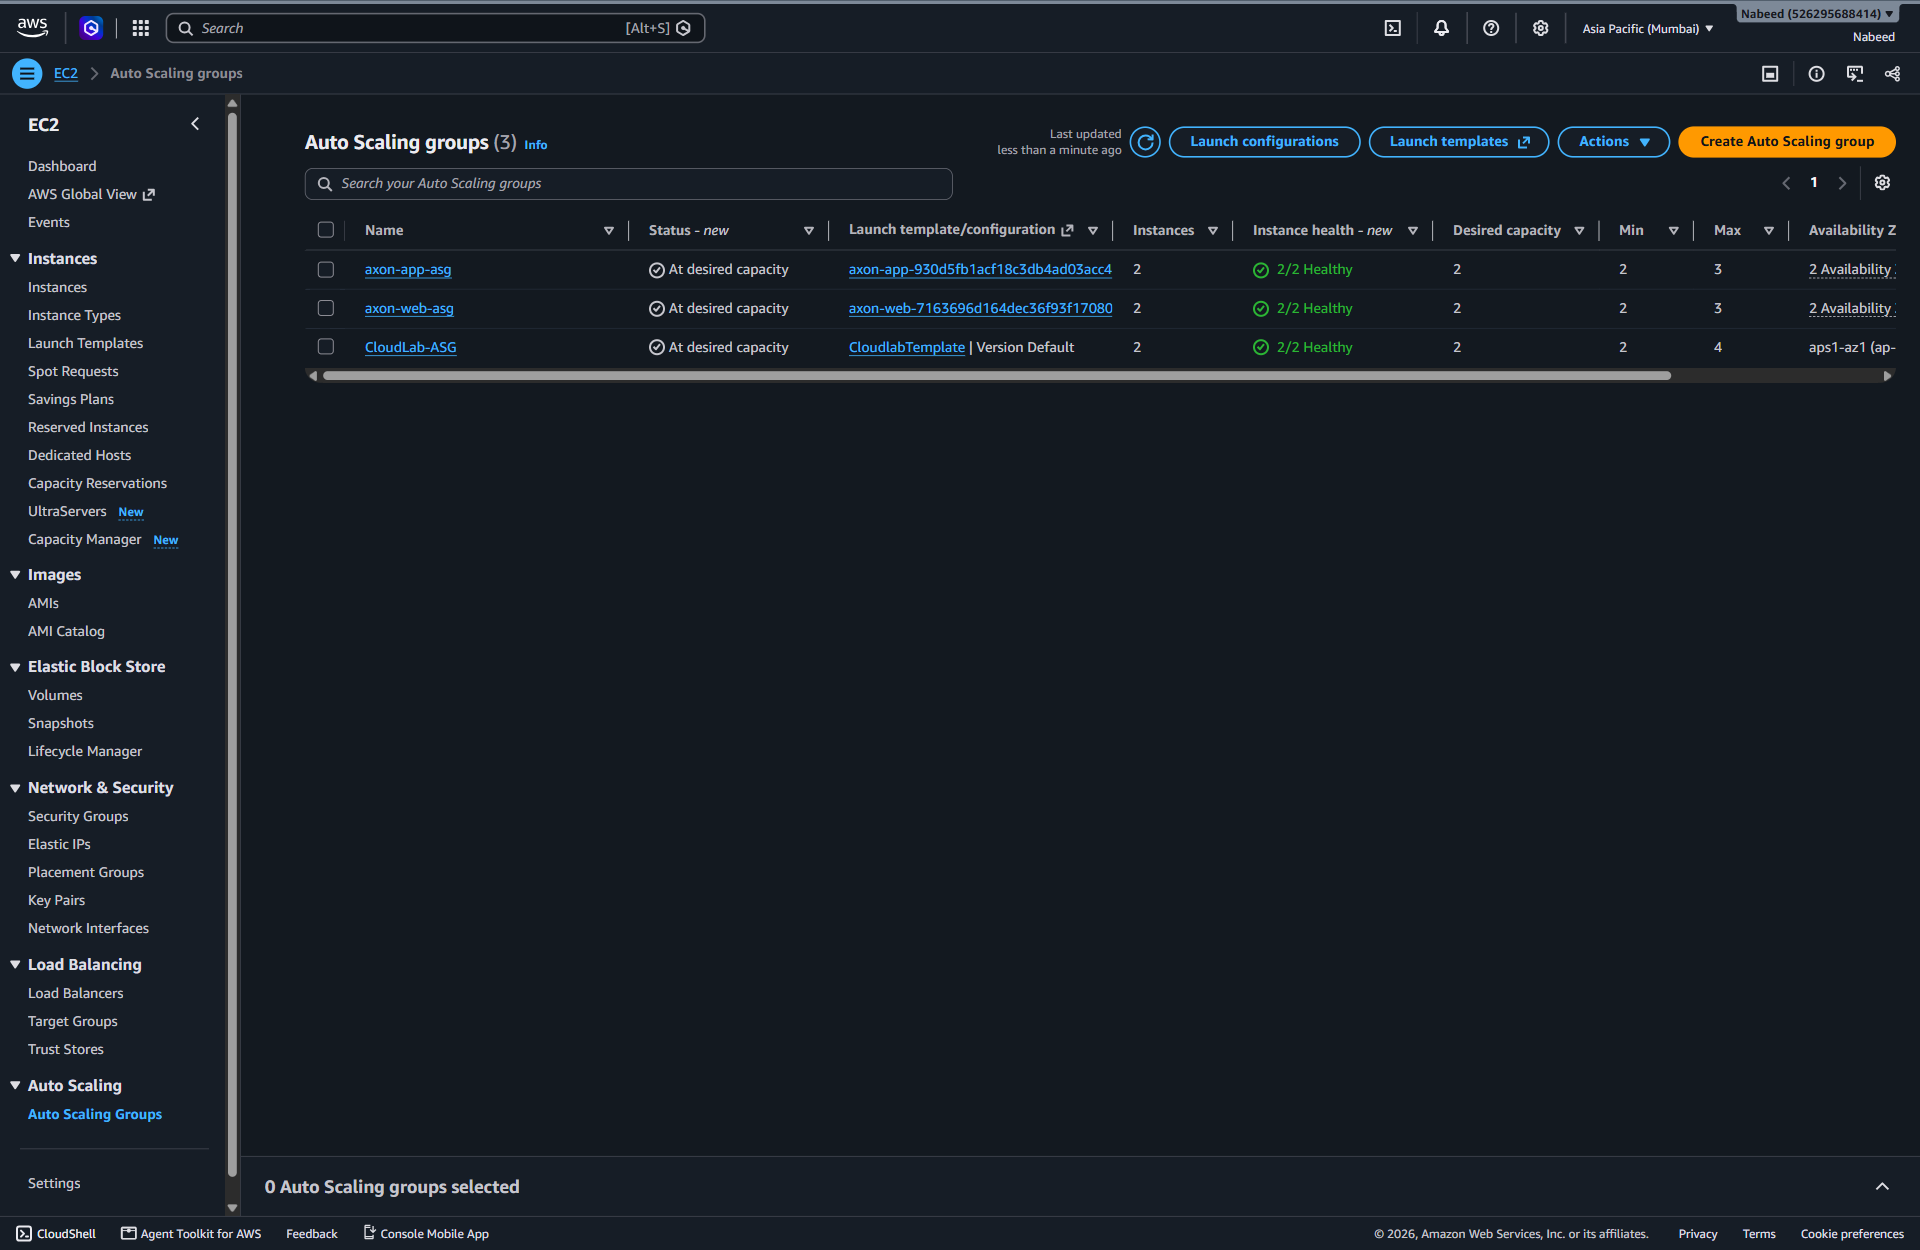
\includegraphics[width=\textwidth]{images/09-auto-scaling-groups.png}\caption{Auto Scaling groups for the web and app tiers.}\end{figure}
\begin{figure}[H]\centering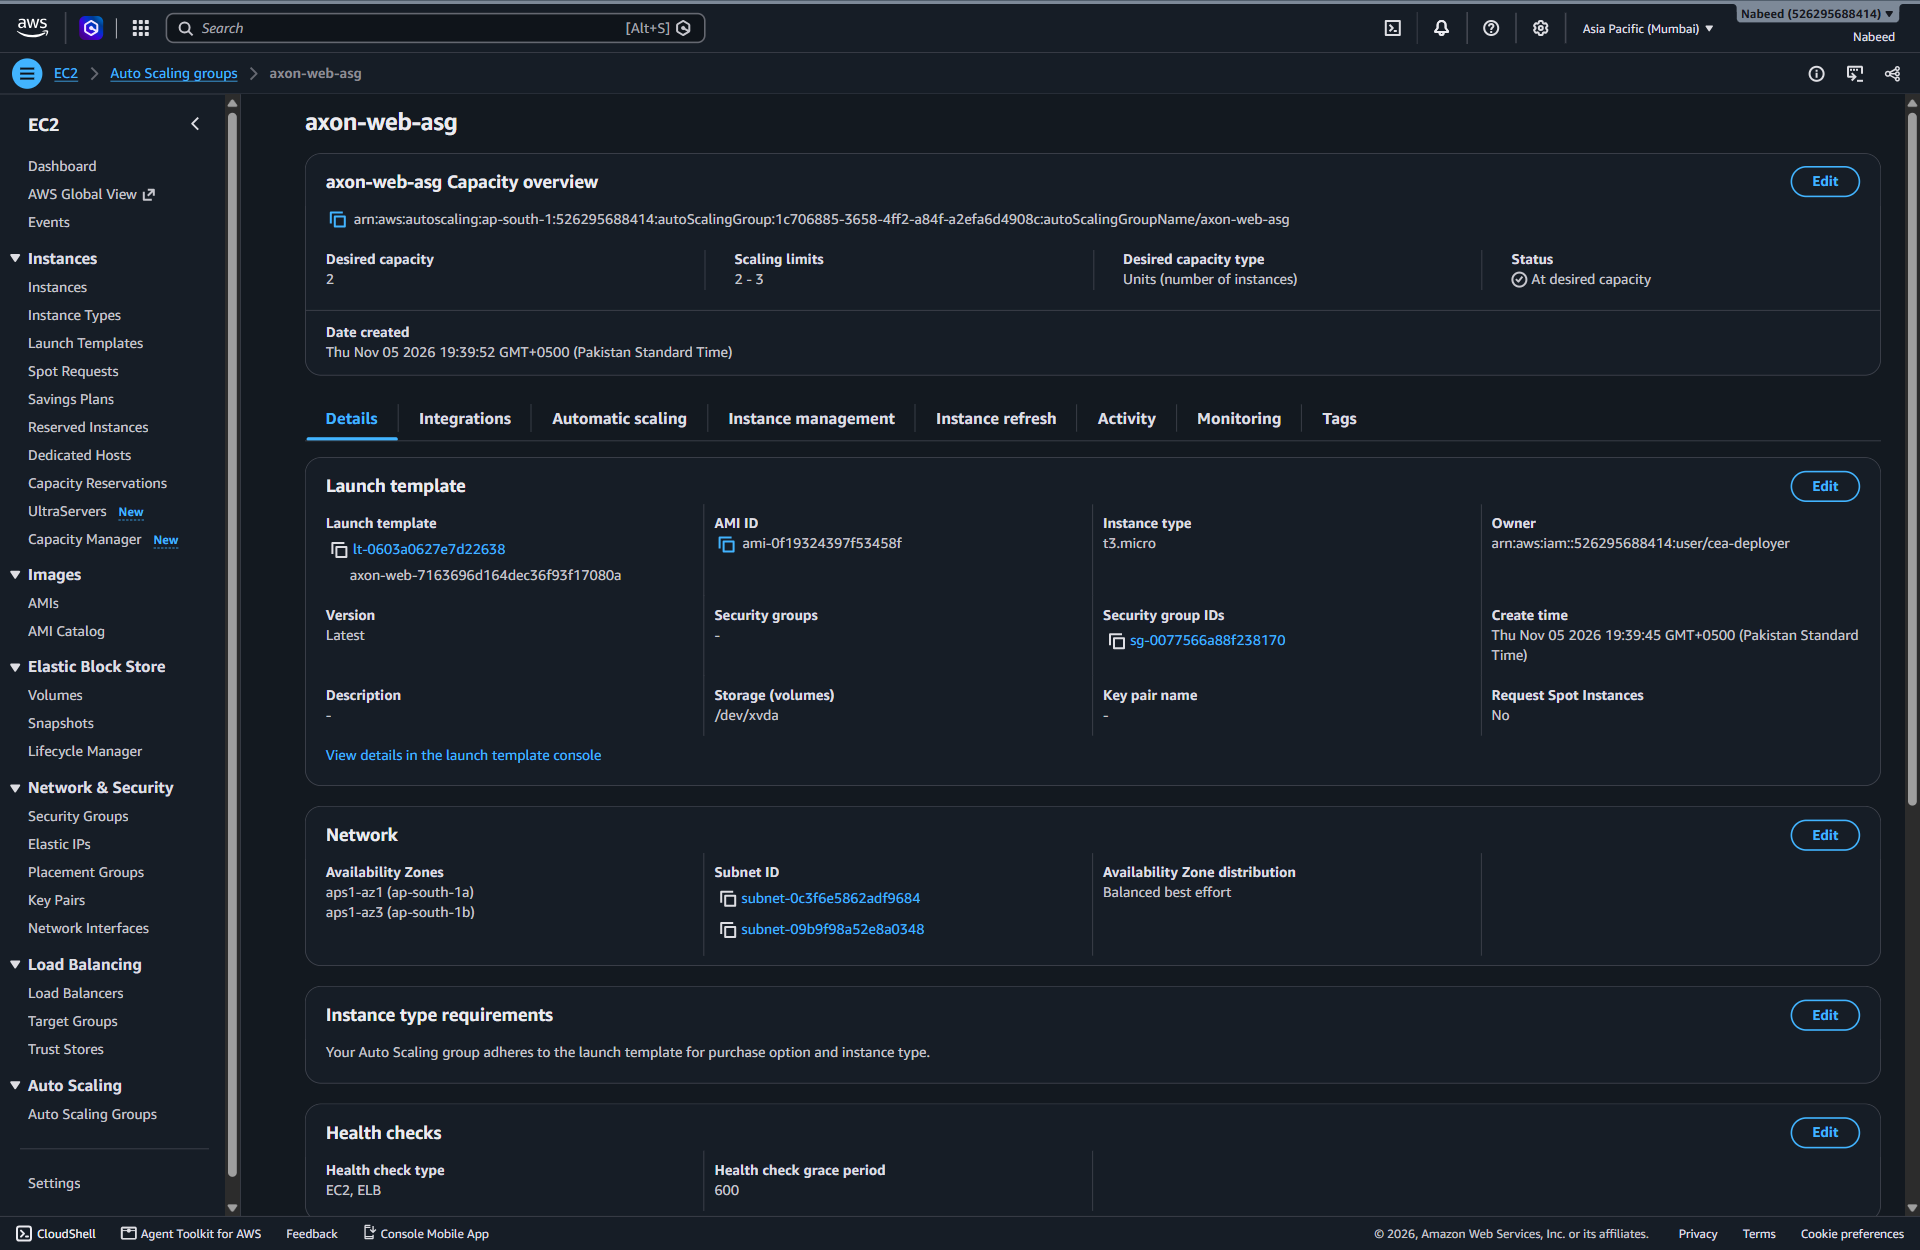
\includegraphics[width=\textwidth]{images/26-web-asg-detail.png}\caption{Web ASG details: capacity, launch template and target group.}\end{figure}
\section*{Security groups / firewall rules}
\begin{figure}[H]\centering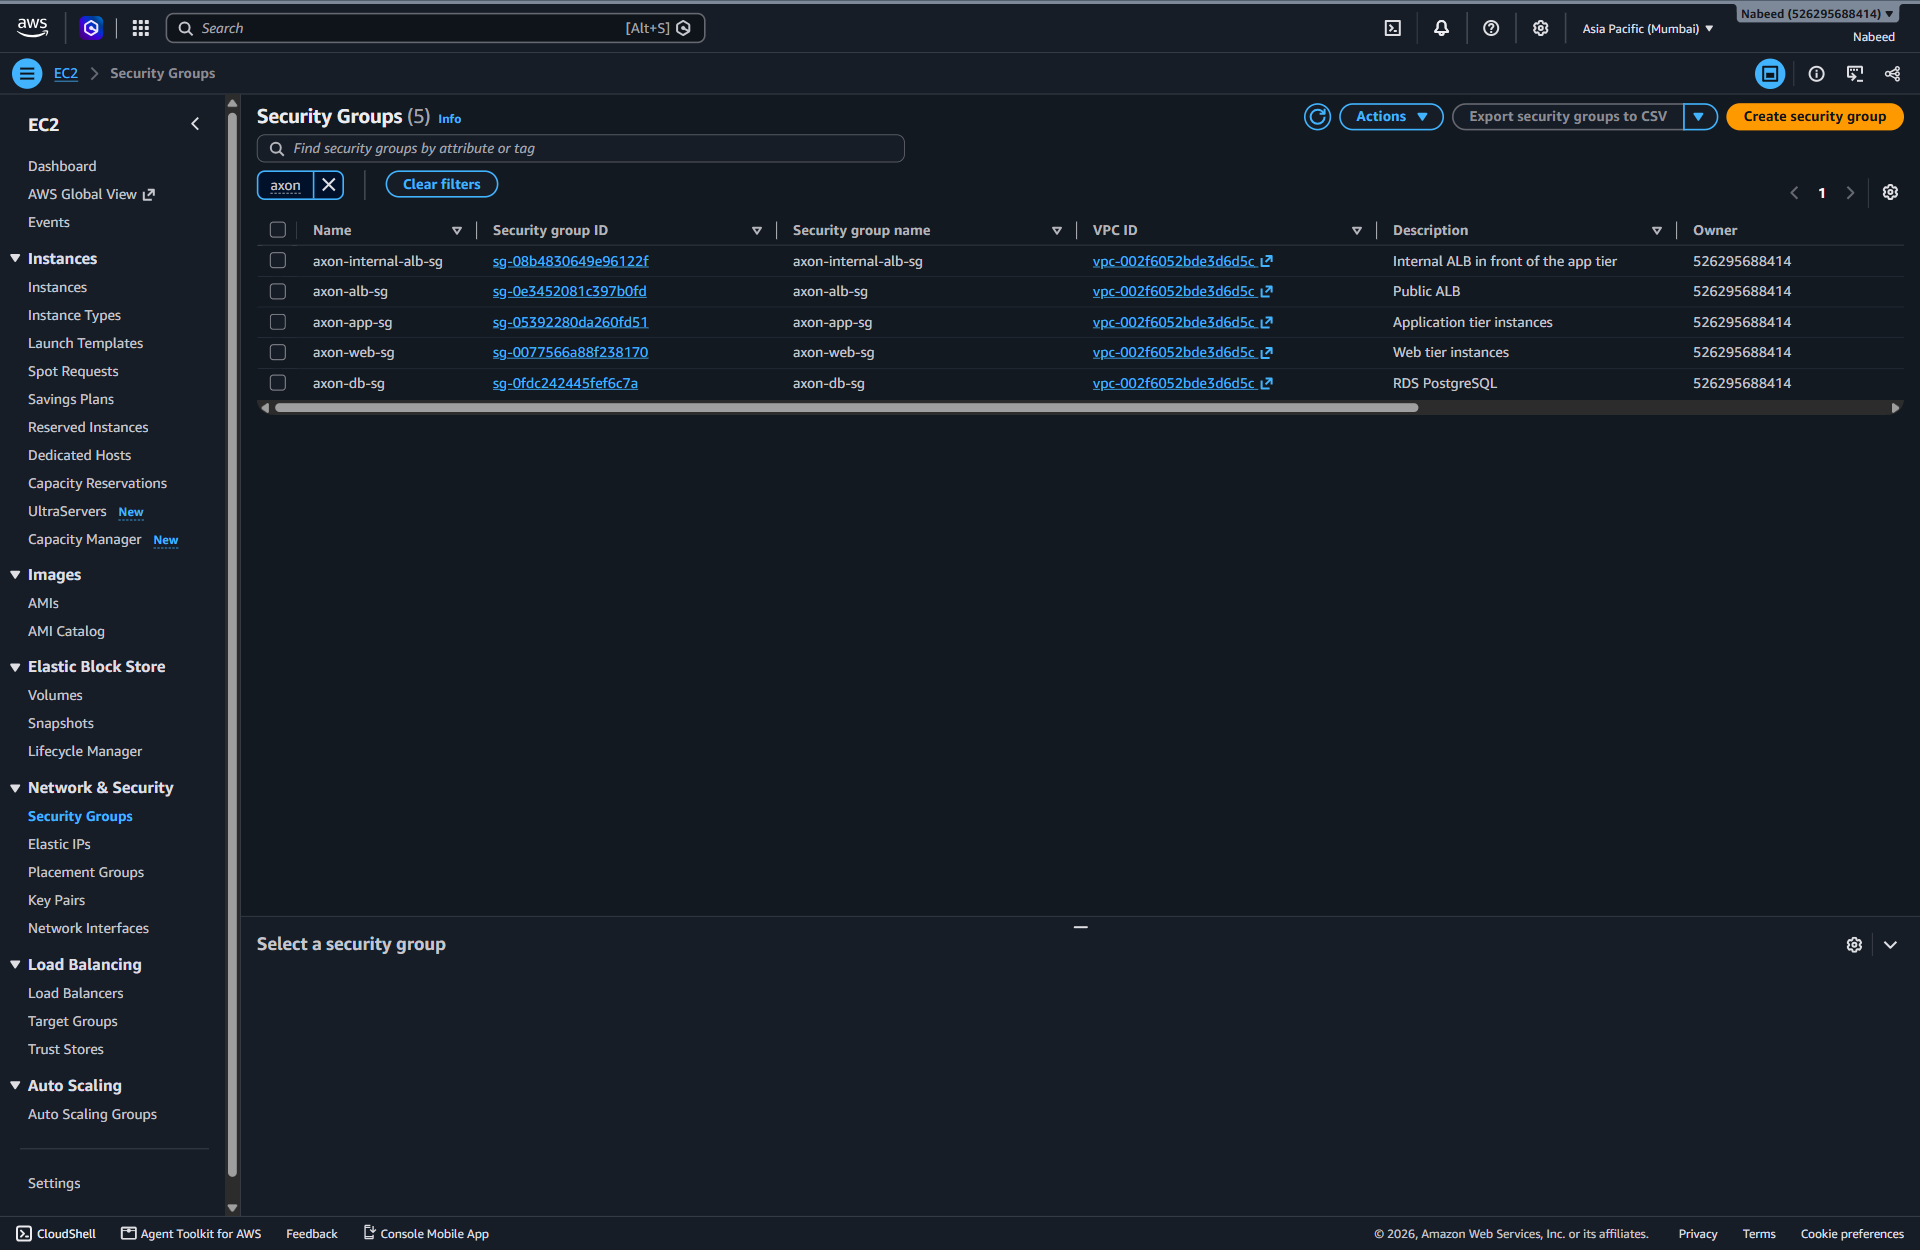
\includegraphics[width=\textwidth]{images/06-security-groups.png}\caption{One security group per tier.}\end{figure}
\begin{figure}[H]\centering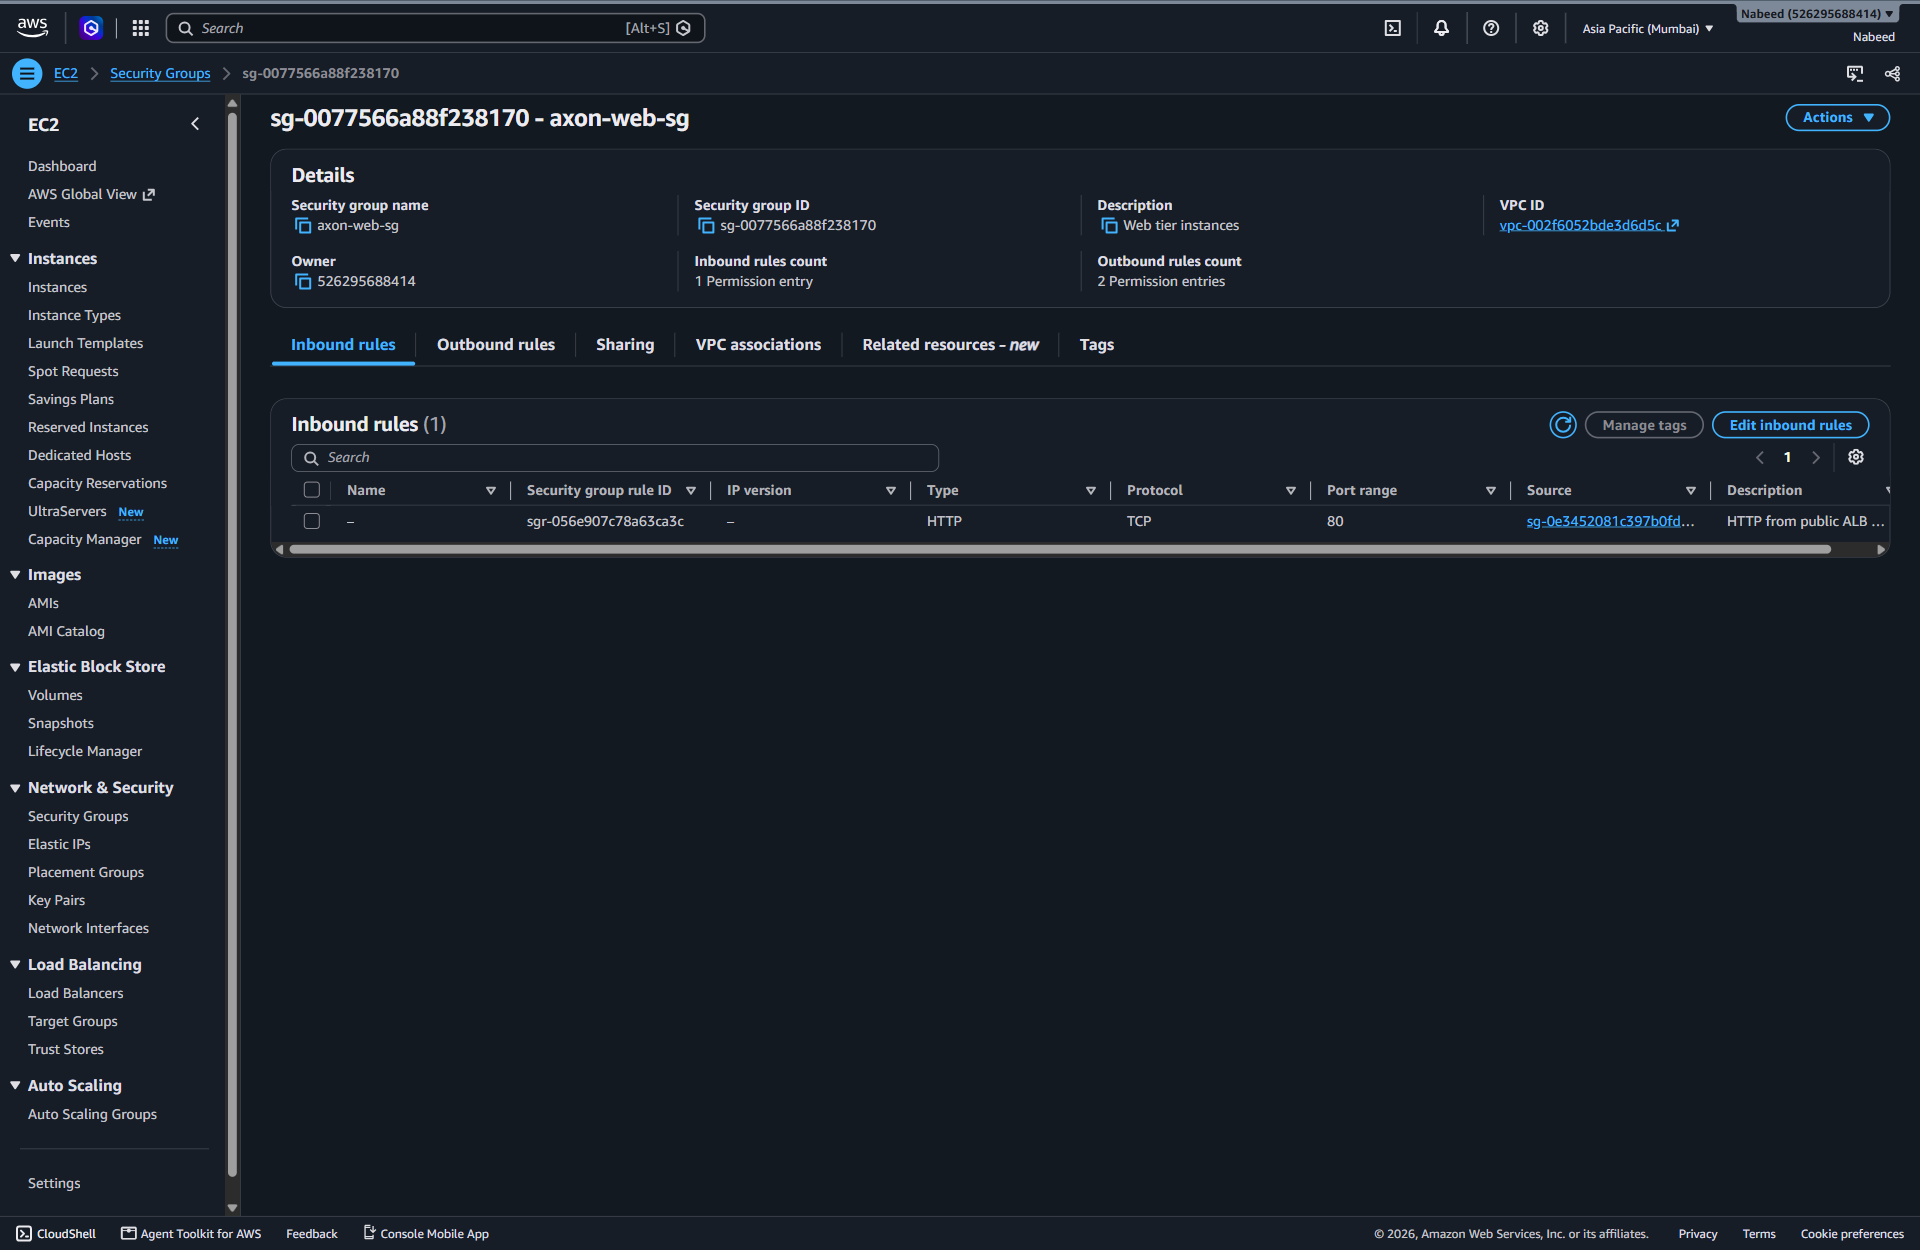
\includegraphics[width=\textwidth]{images/17-sg-web-rules.png}\caption{Web tier: inbound HTTP only from the public ALB security group.}\end{figure}
\begin{figure}[H]\centering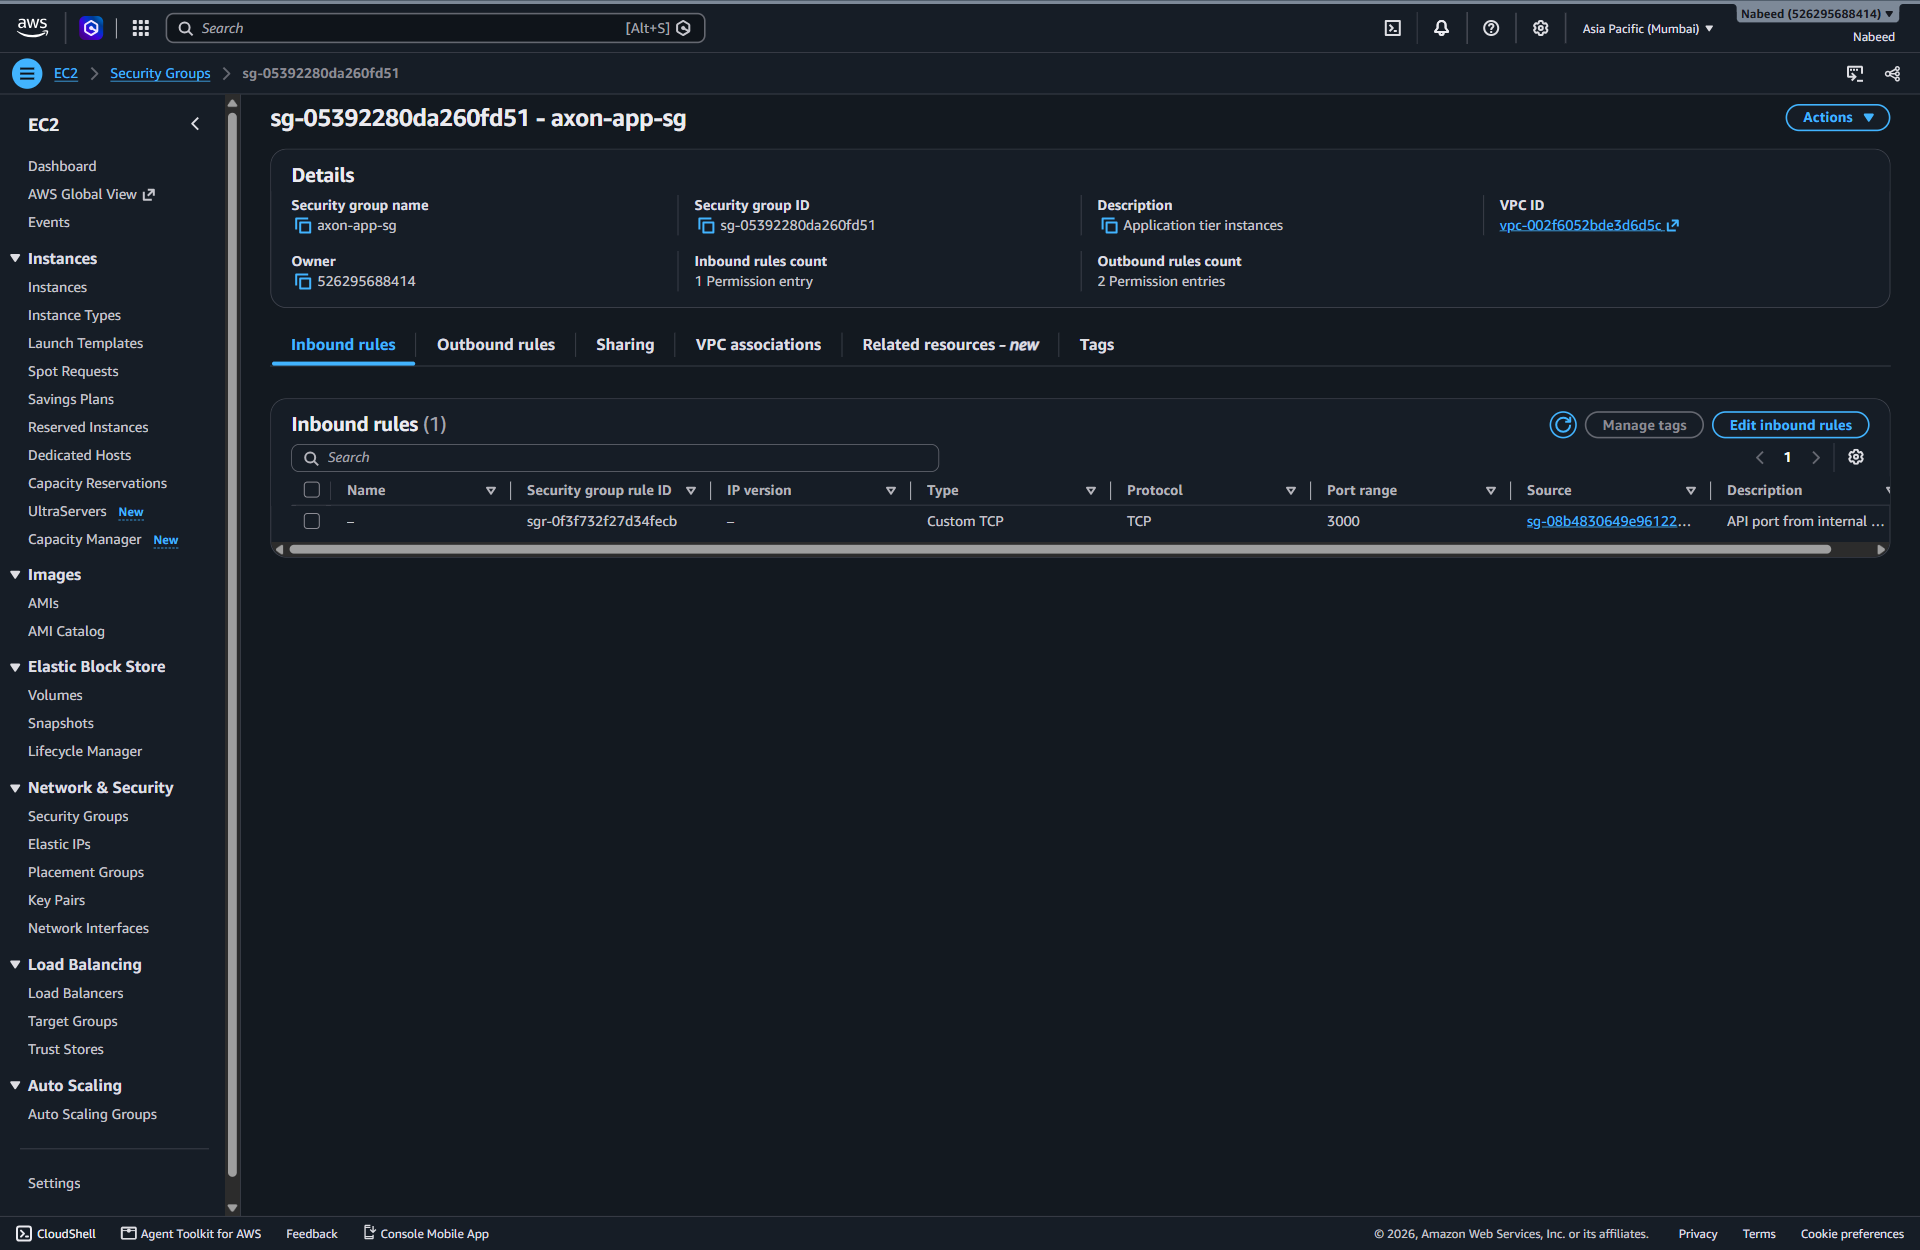
\includegraphics[width=\textwidth]{images/18-sg-app-rules.png}\caption{App tier: inbound 3000 only from the internal ALB security group.}\end{figure}
\begin{figure}[H]\centering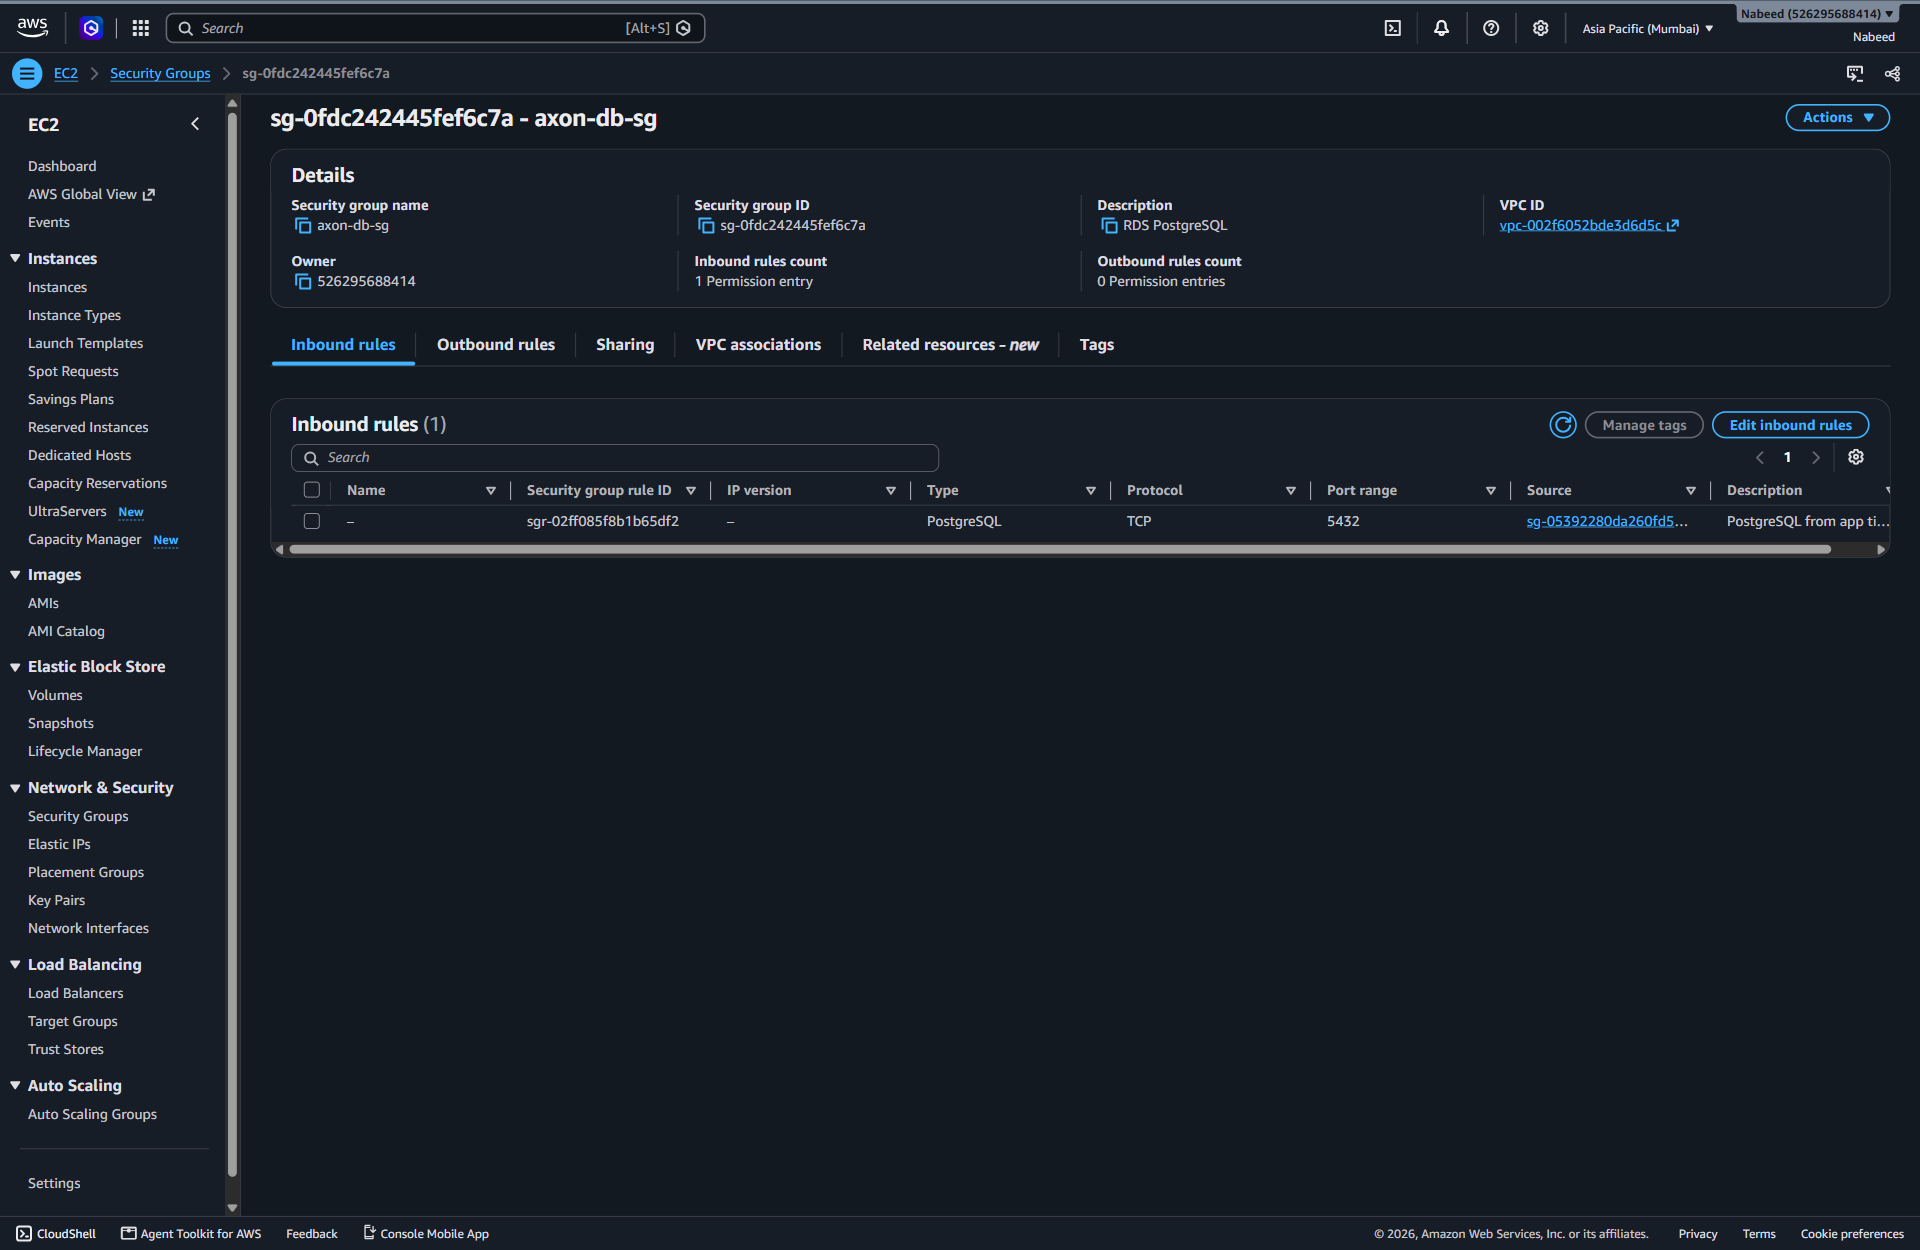
\includegraphics[width=\textwidth]{images/19-sg-db-rules.png}\caption{DB tier: inbound 5432 only from the app tier security group.}\end{figure}
\begin{figure}[H]\centering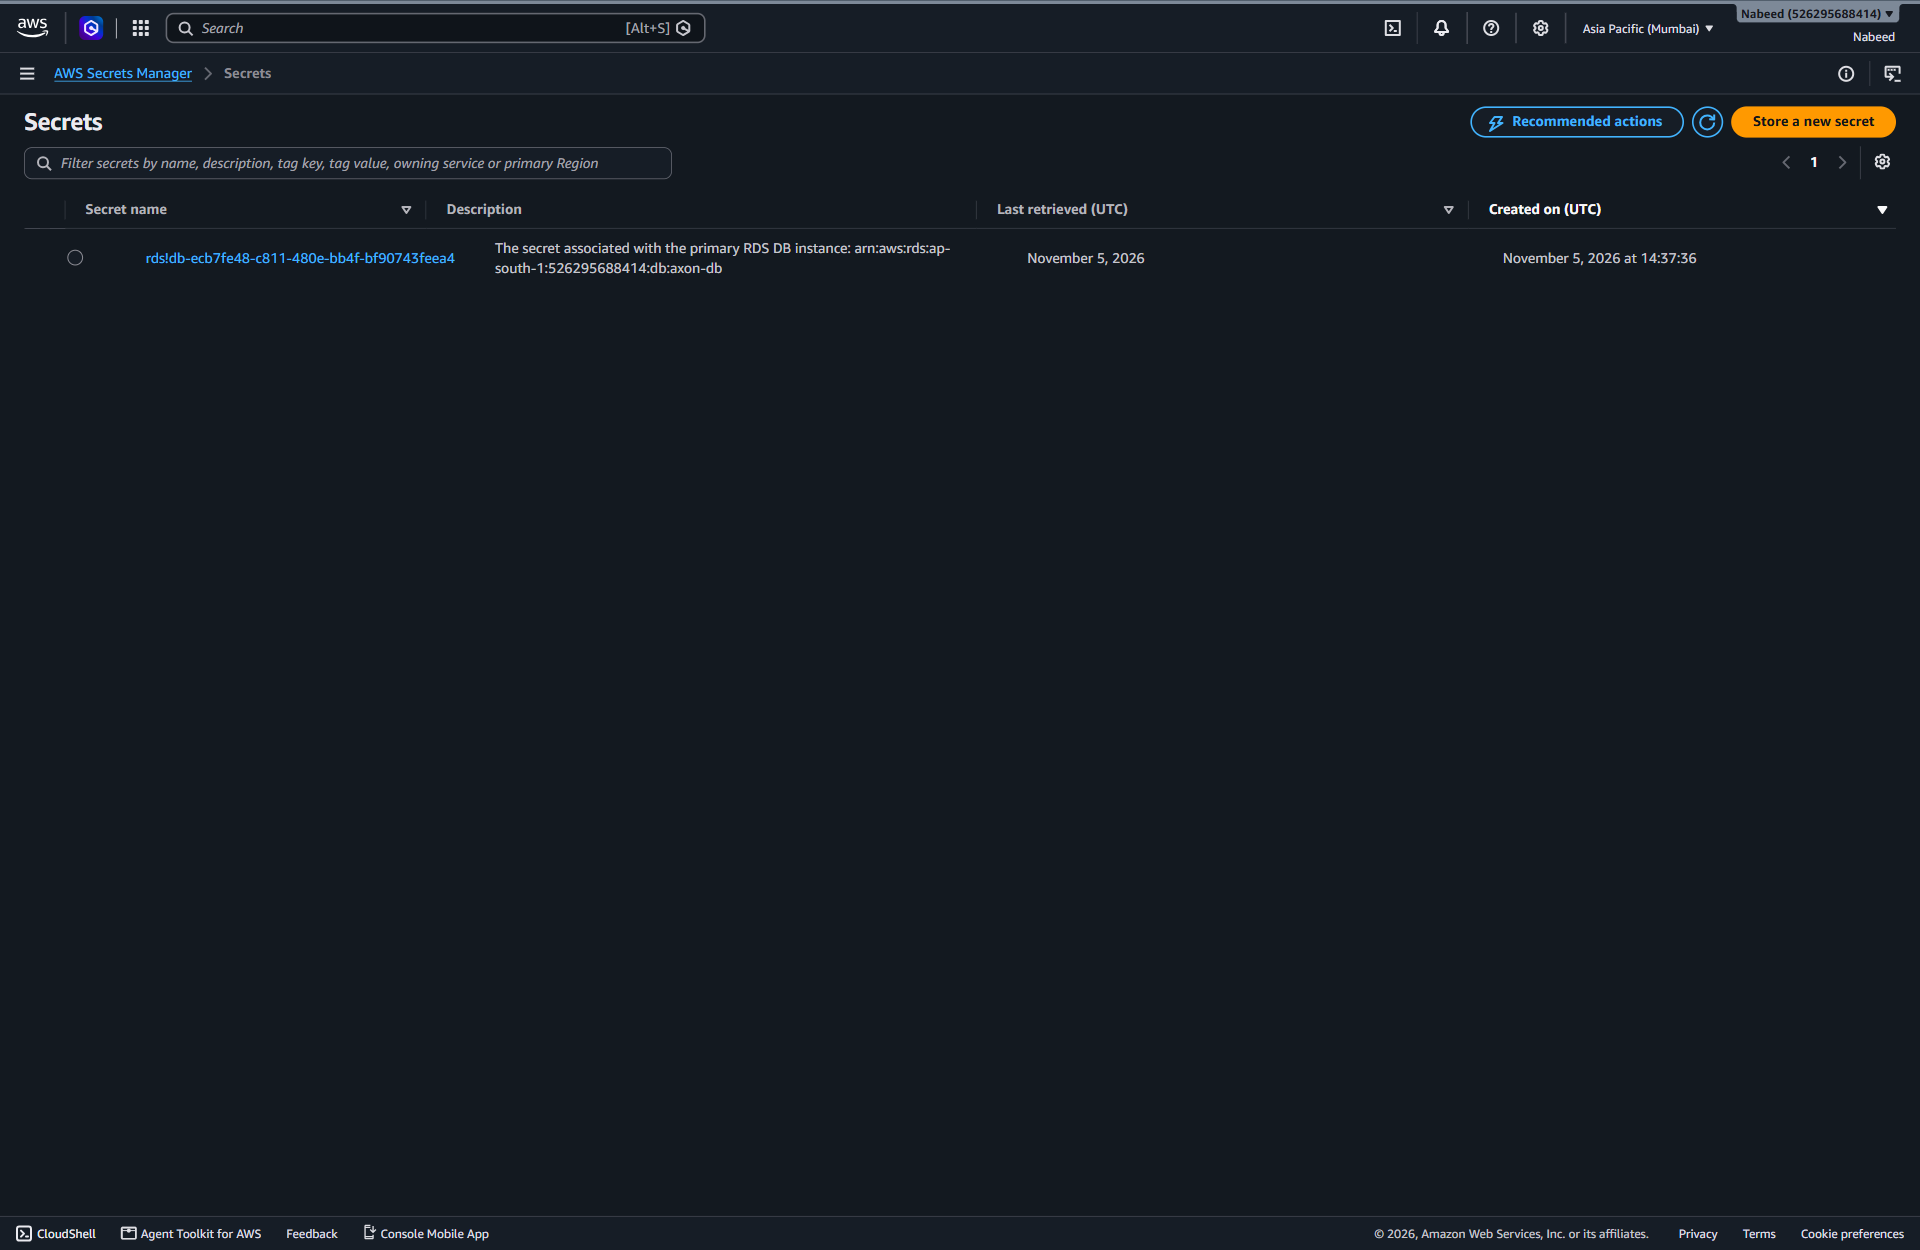
\includegraphics[width=\textwidth]{images/24-secrets-manager.png}\caption{Secrets Manager holds the RDS-managed database credential.}\end{figure}
\section*{Load balancer configuration}
\begin{figure}[H]\centering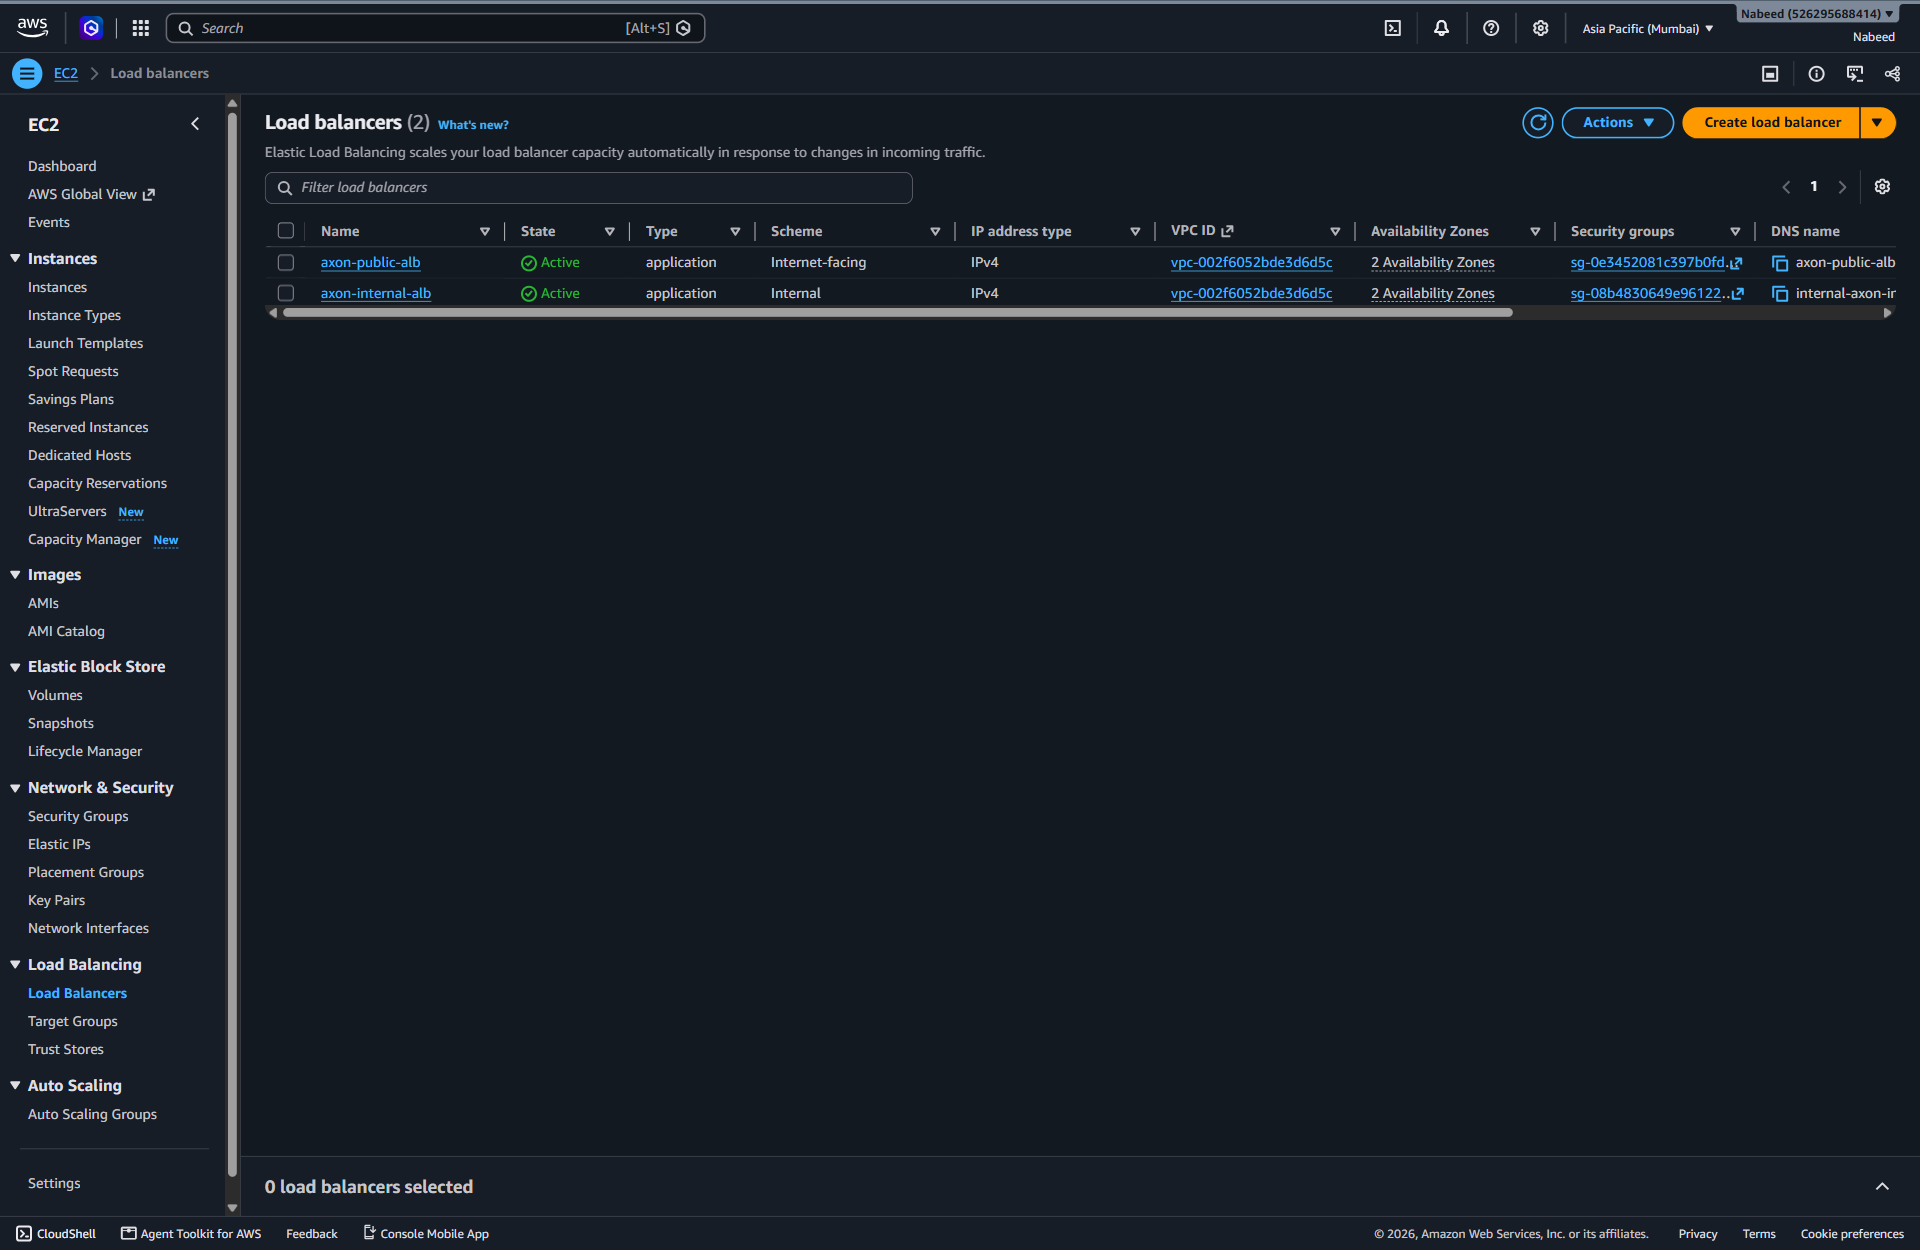
\includegraphics[width=\textwidth]{images/07-load-balancers.png}\caption{Public and internal Application Load Balancers.}\end{figure}
\begin{figure}[H]\centering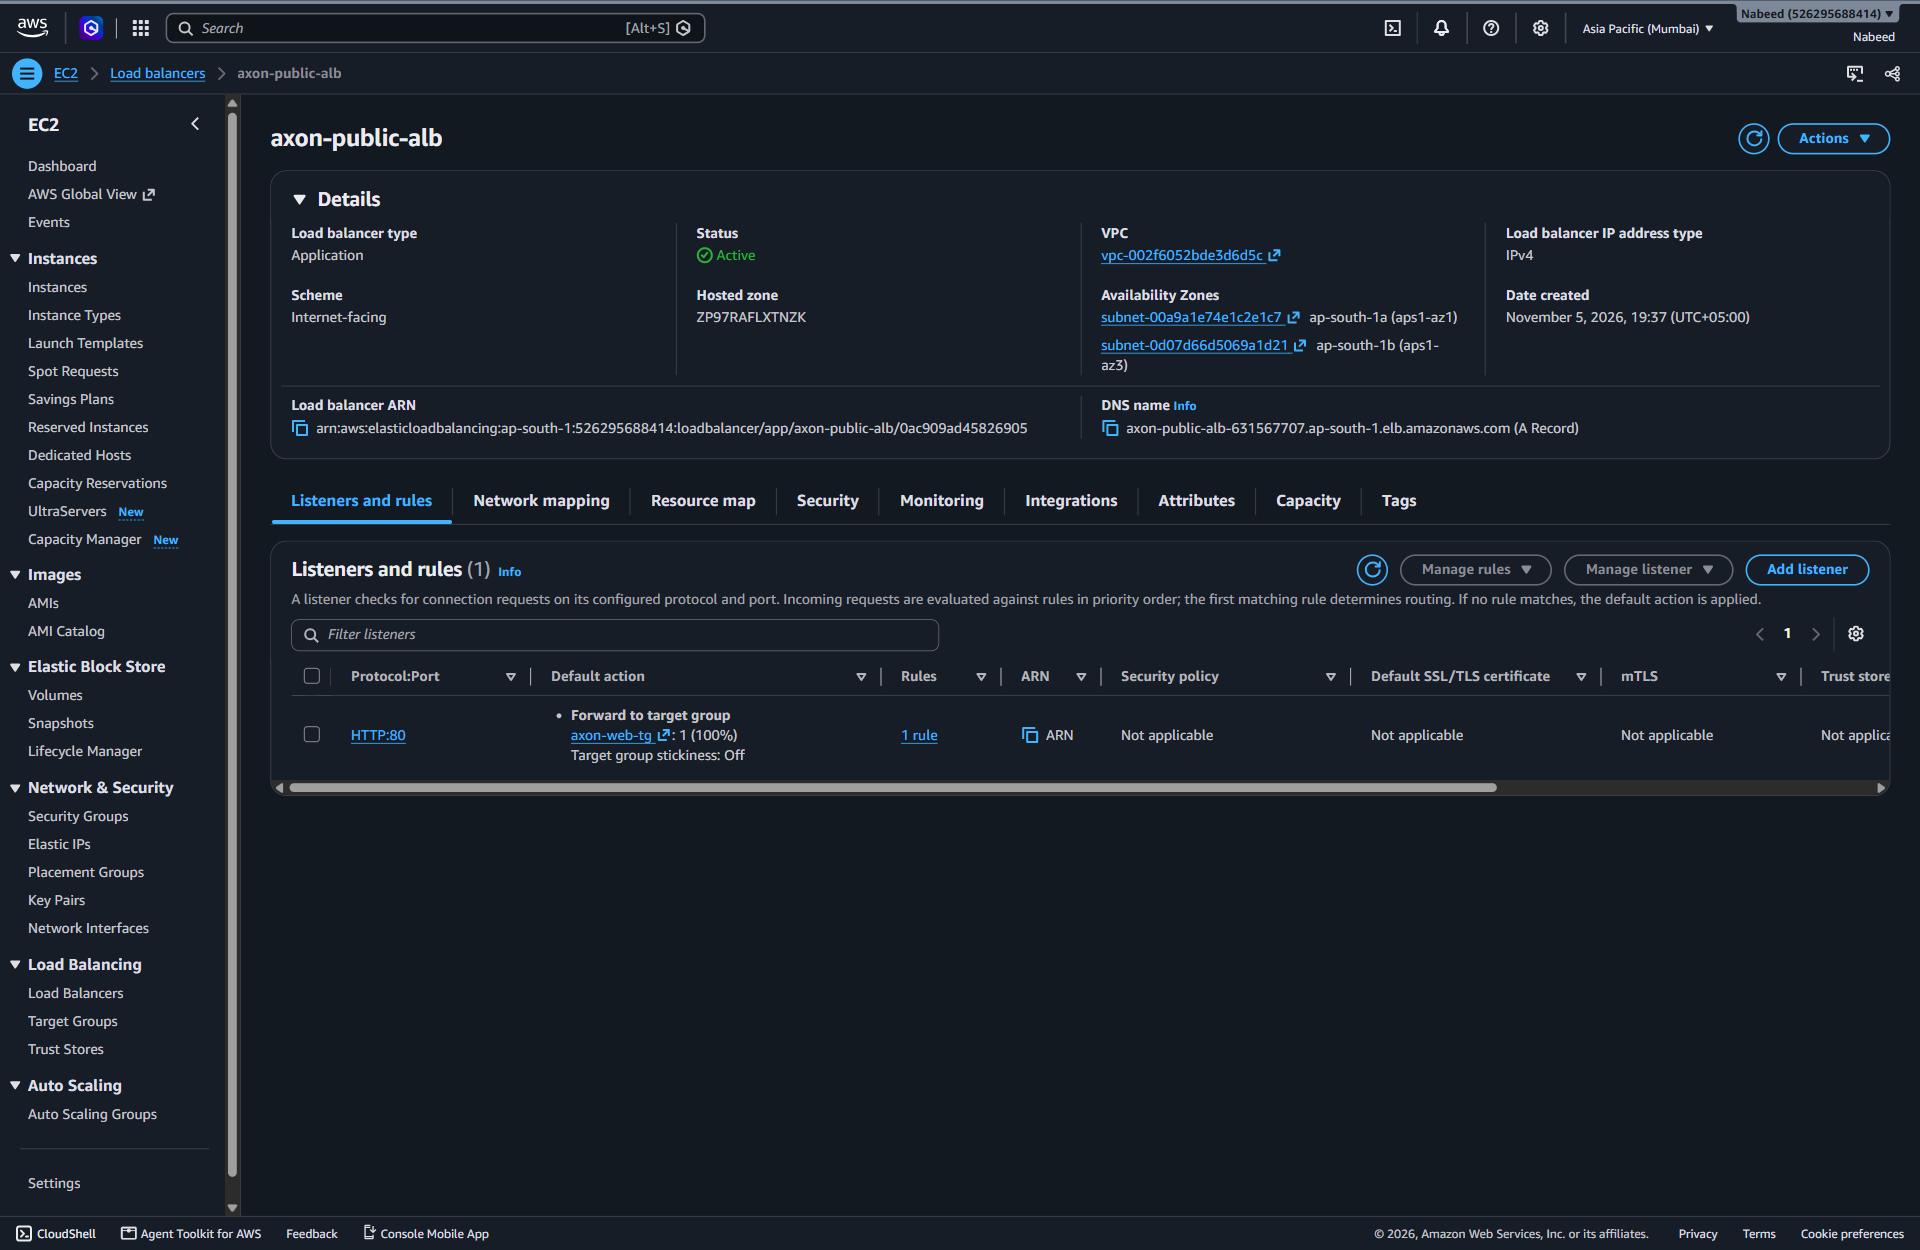
\includegraphics[width=\textwidth]{images/25-public-alb-detail.png}\caption{Public ALB detail: listener, subnets, security group.}\end{figure}
\begin{figure}[H]\centering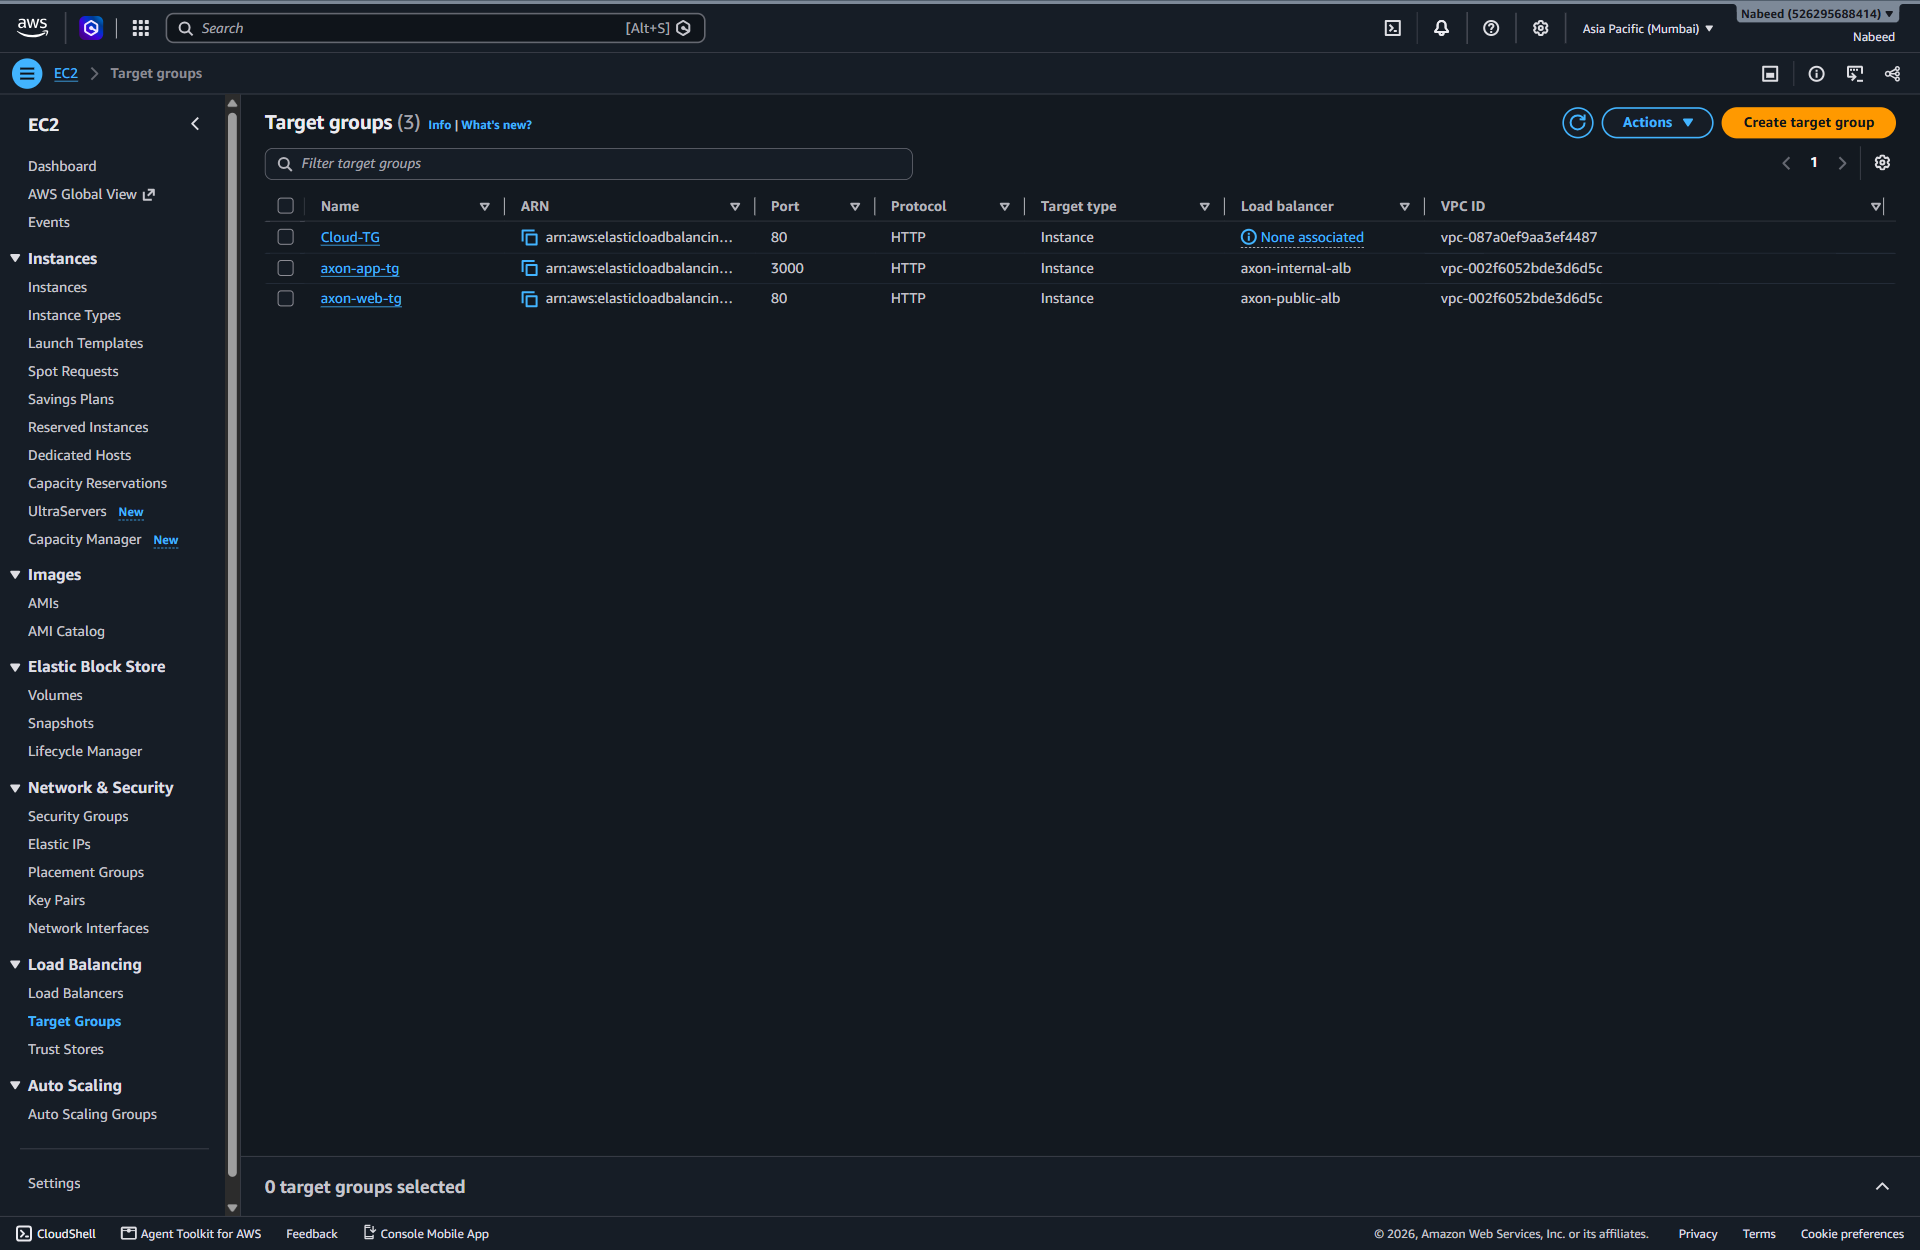
\includegraphics[width=\textwidth]{images/08-target-groups.png}\caption{Target groups (web :80, app :3000) with healthy targets.}\end{figure}
\section*{Database instance}
\begin{figure}[H]\centering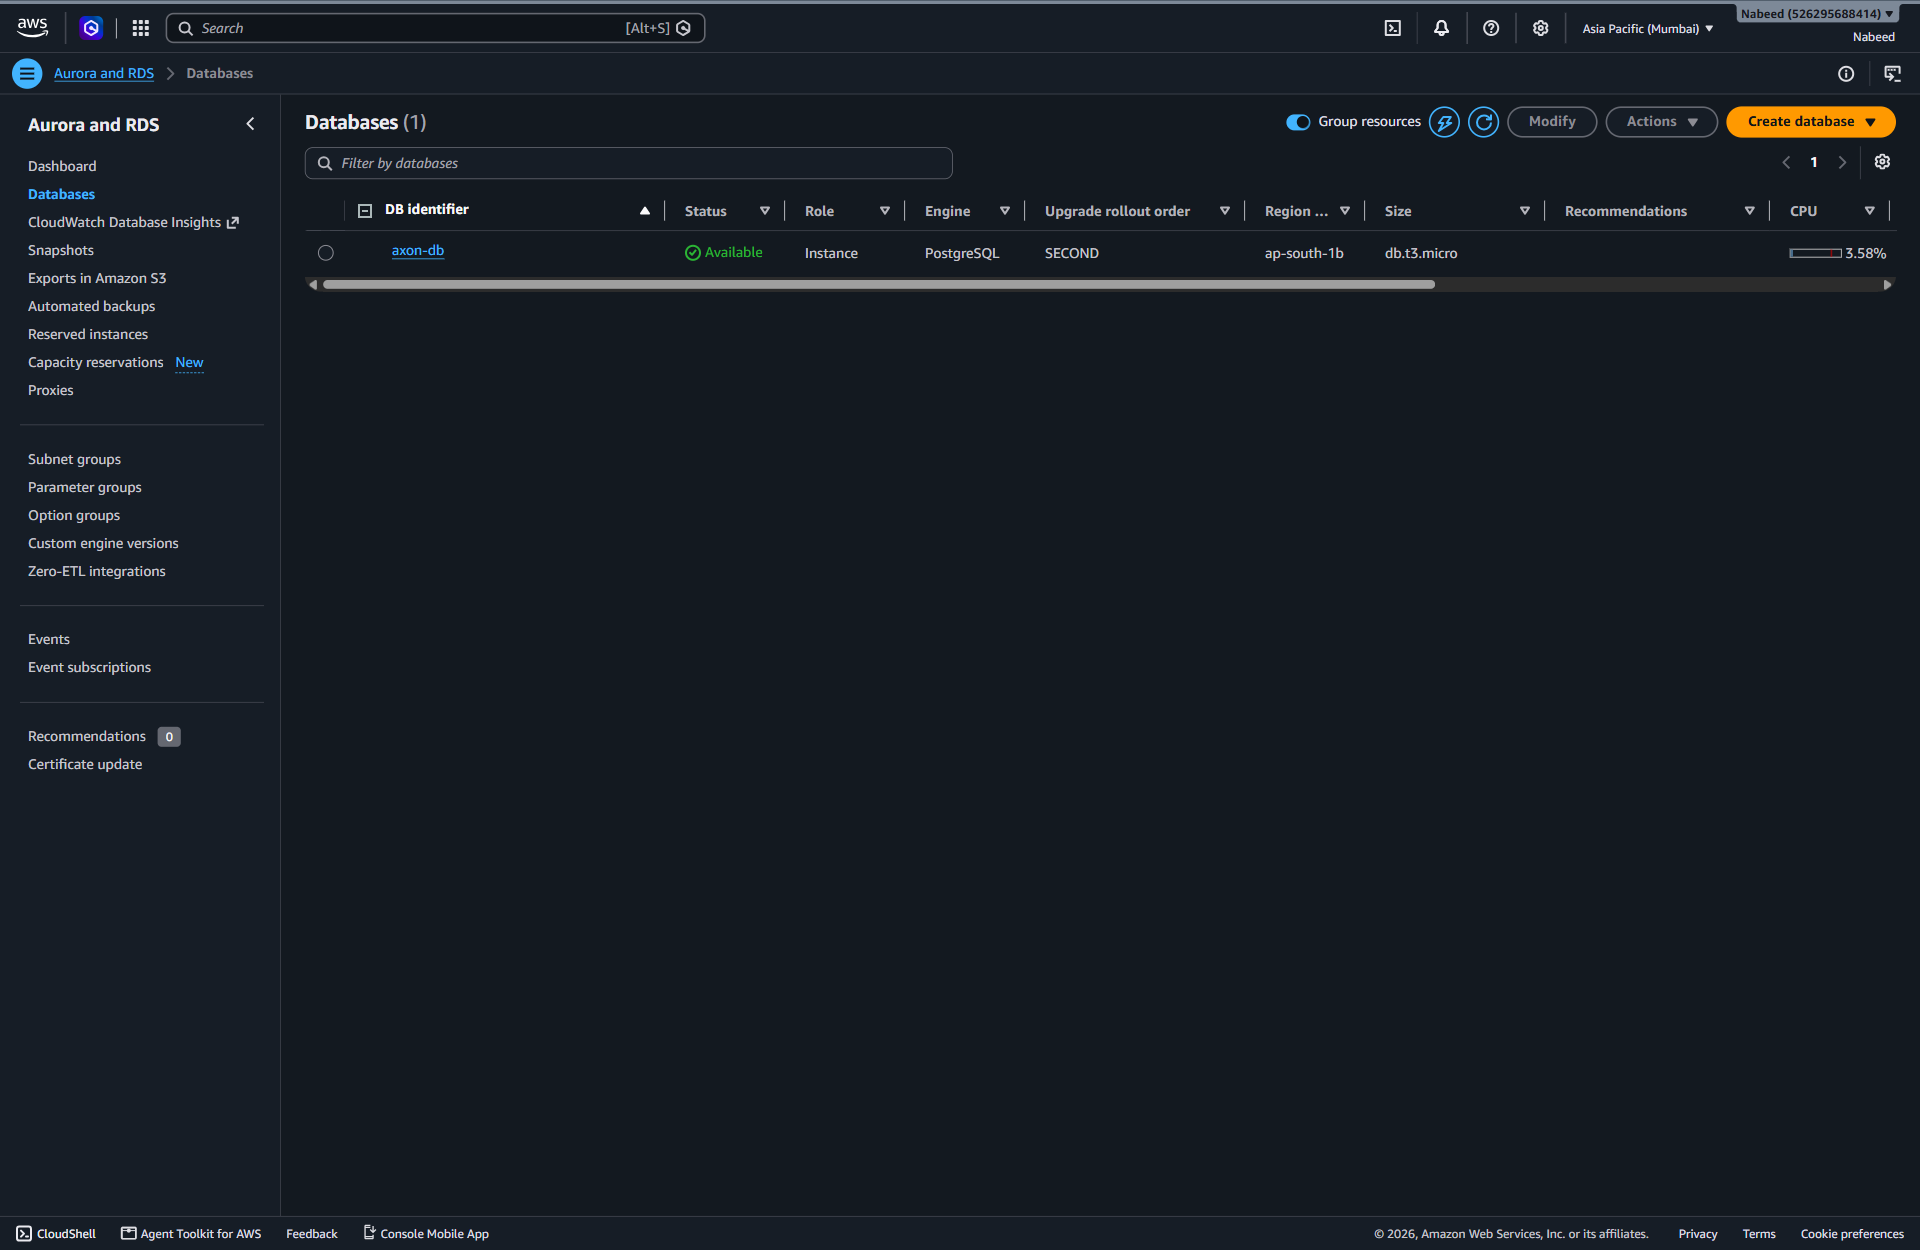
\includegraphics[width=\textwidth]{images/10-rds-database.png}\caption{RDS PostgreSQL instance \texttt{axon-db} (available).}\end{figure}
\begin{figure}[H]\centering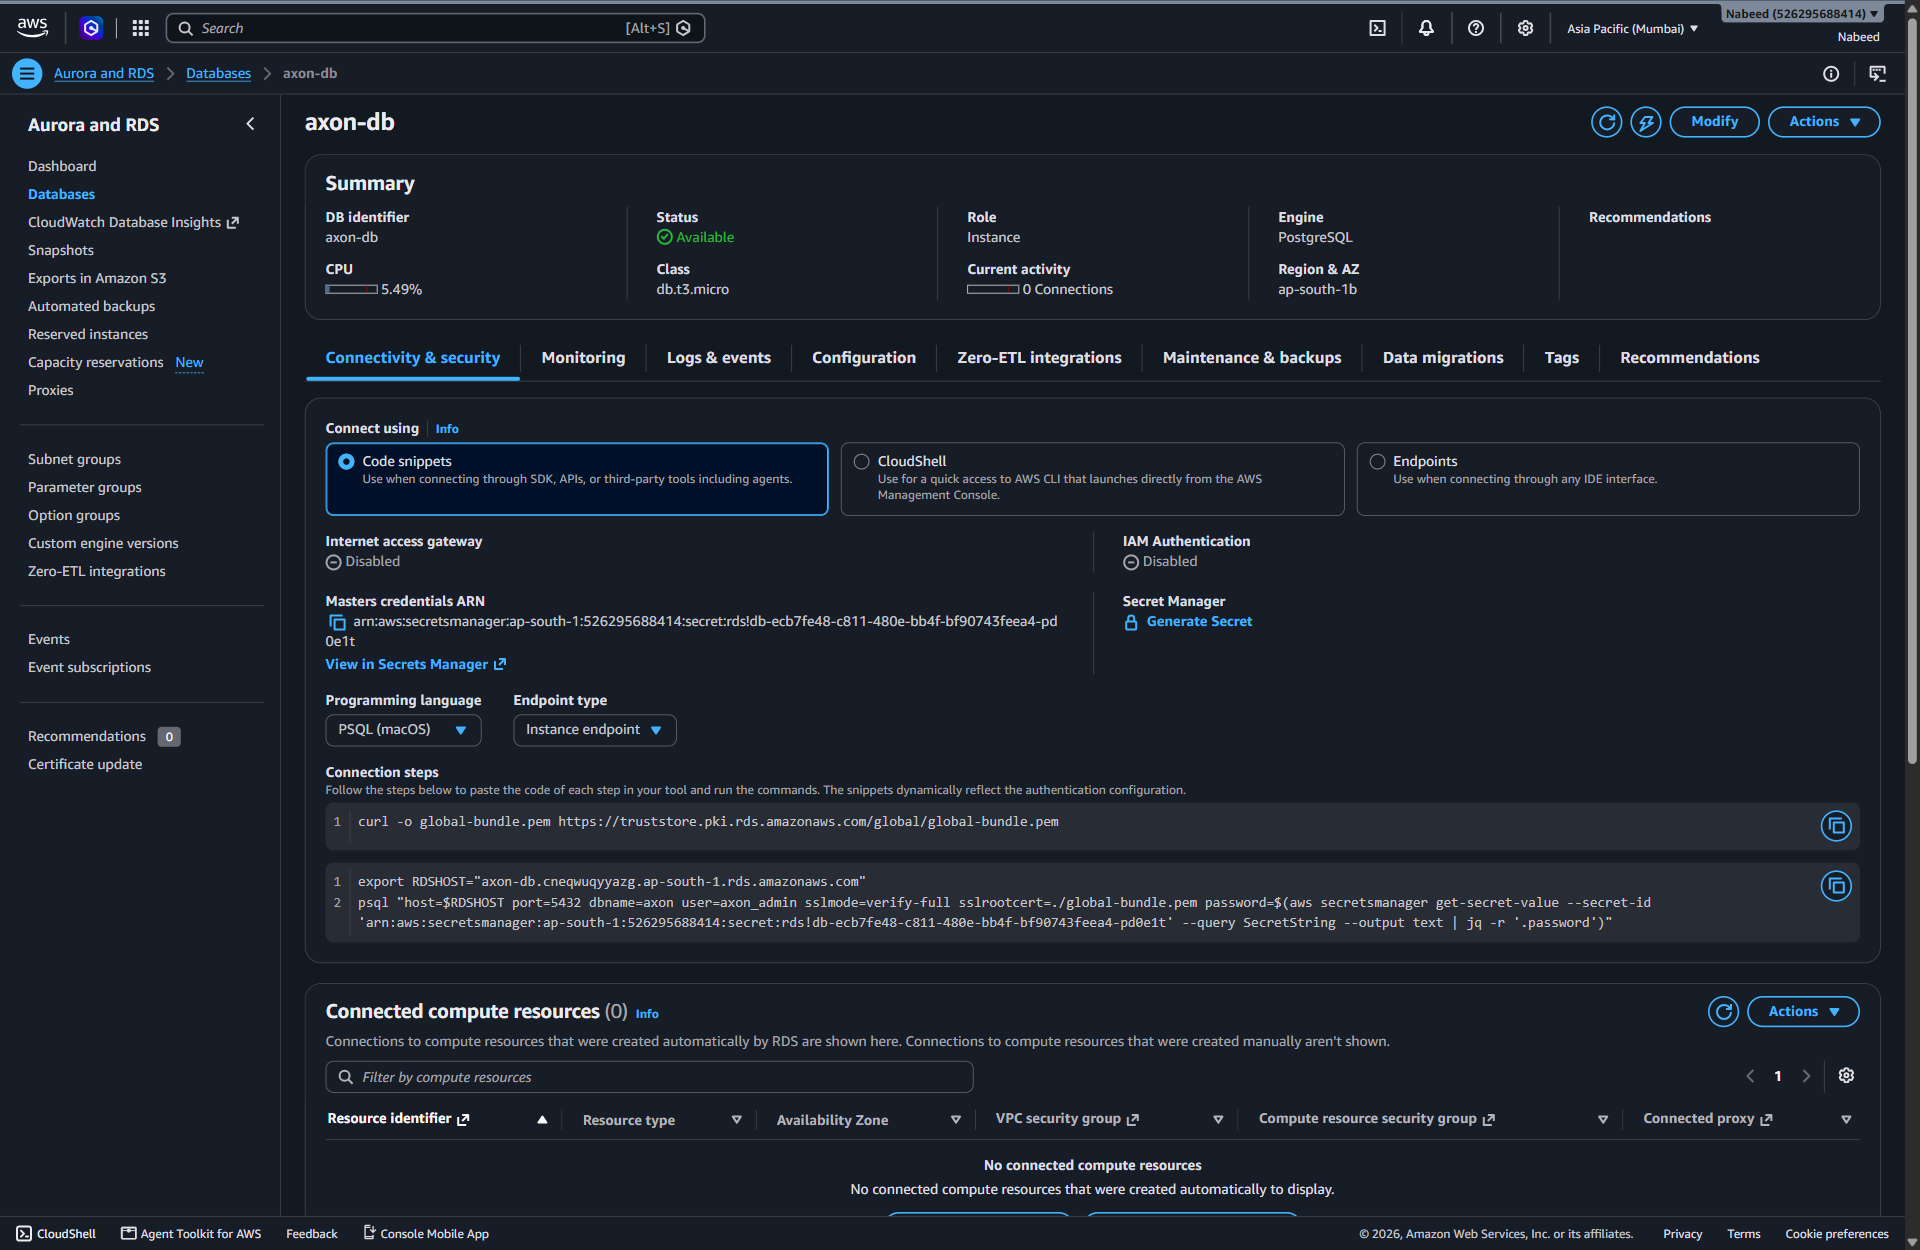
\includegraphics[width=\textwidth]{images/20-rds-detail.png}\caption{RDS detail: private, not publicly accessible, VPC security group.}\end{figure}
\section*{Docker image build and registry listing}
\begin{figure}[H]\centering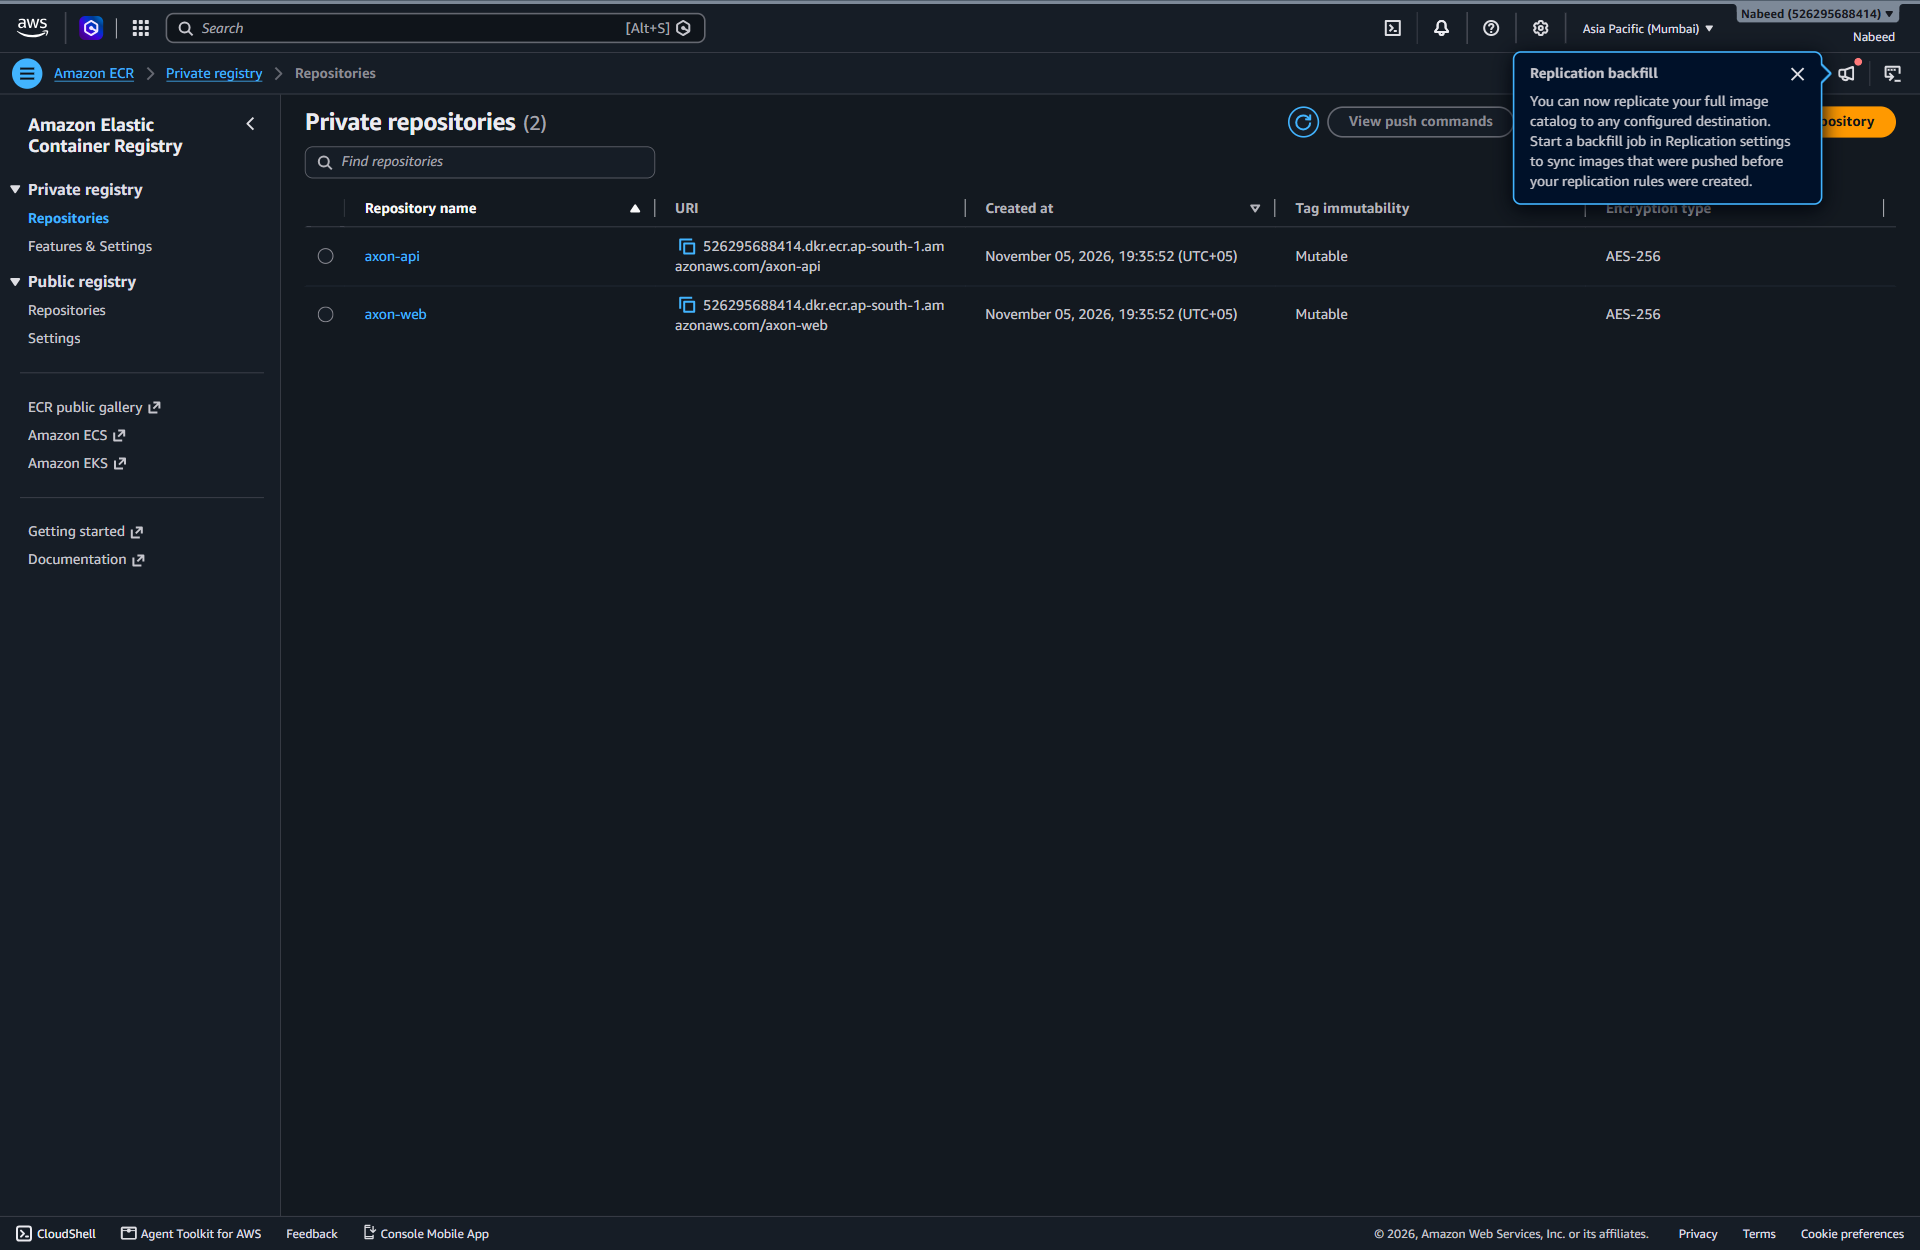
\includegraphics[width=\textwidth]{images/11-ecr-repositories.png}\caption{Amazon ECR repositories.}\end{figure}
\begin{figure}[H]\centering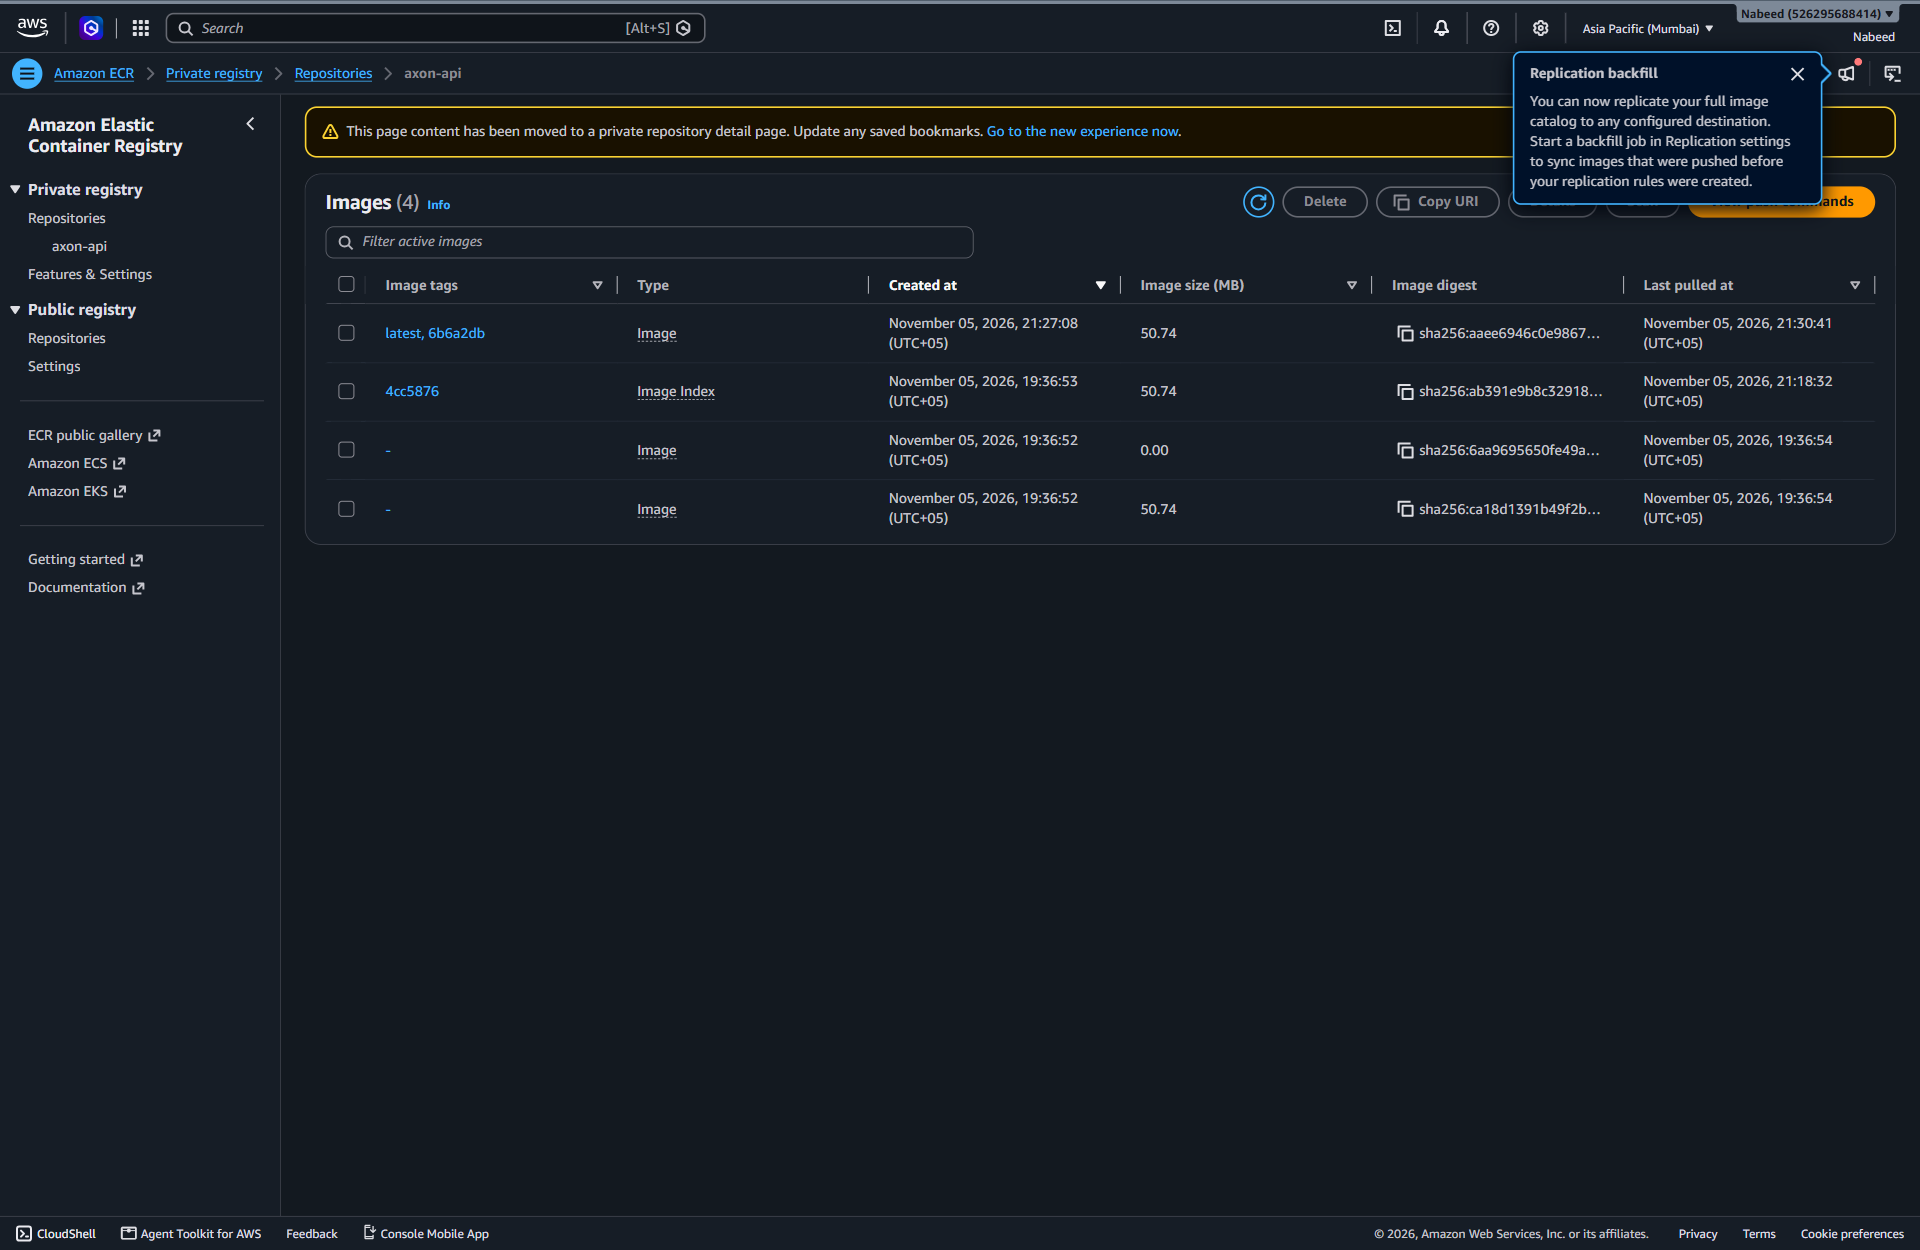
\includegraphics[width=\textwidth]{images/12-ecr-api-images.png}\caption{API images tagged with commit SHA and latest.}\end{figure}
\begin{figure}[H]\centering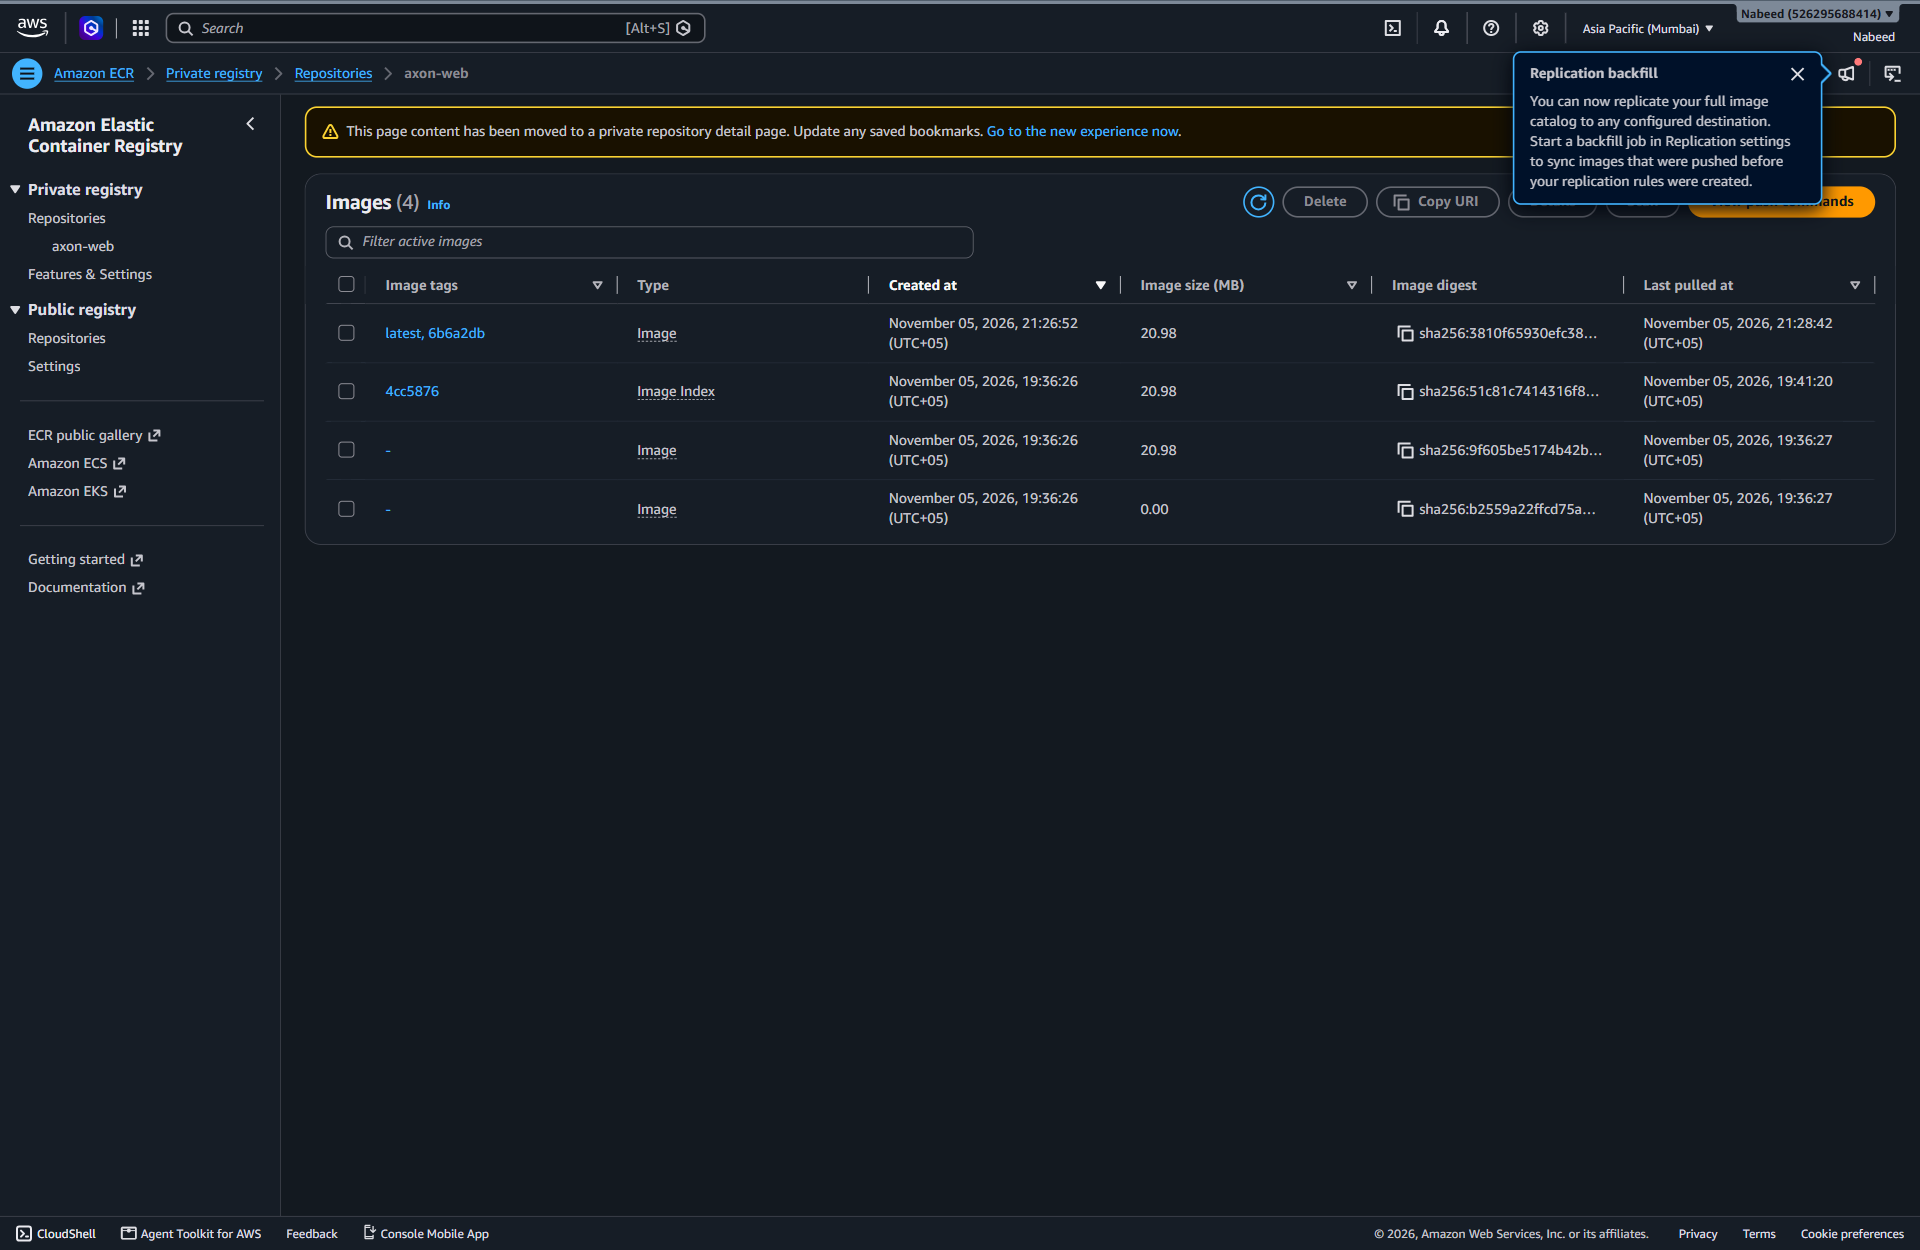
\includegraphics[width=\textwidth]{images/13-ecr-web-images.png}\caption{Web images tagged with commit SHA and latest.}\end{figure}
\section*{CI/CD pipeline run}
\begin{figure}[H]\centering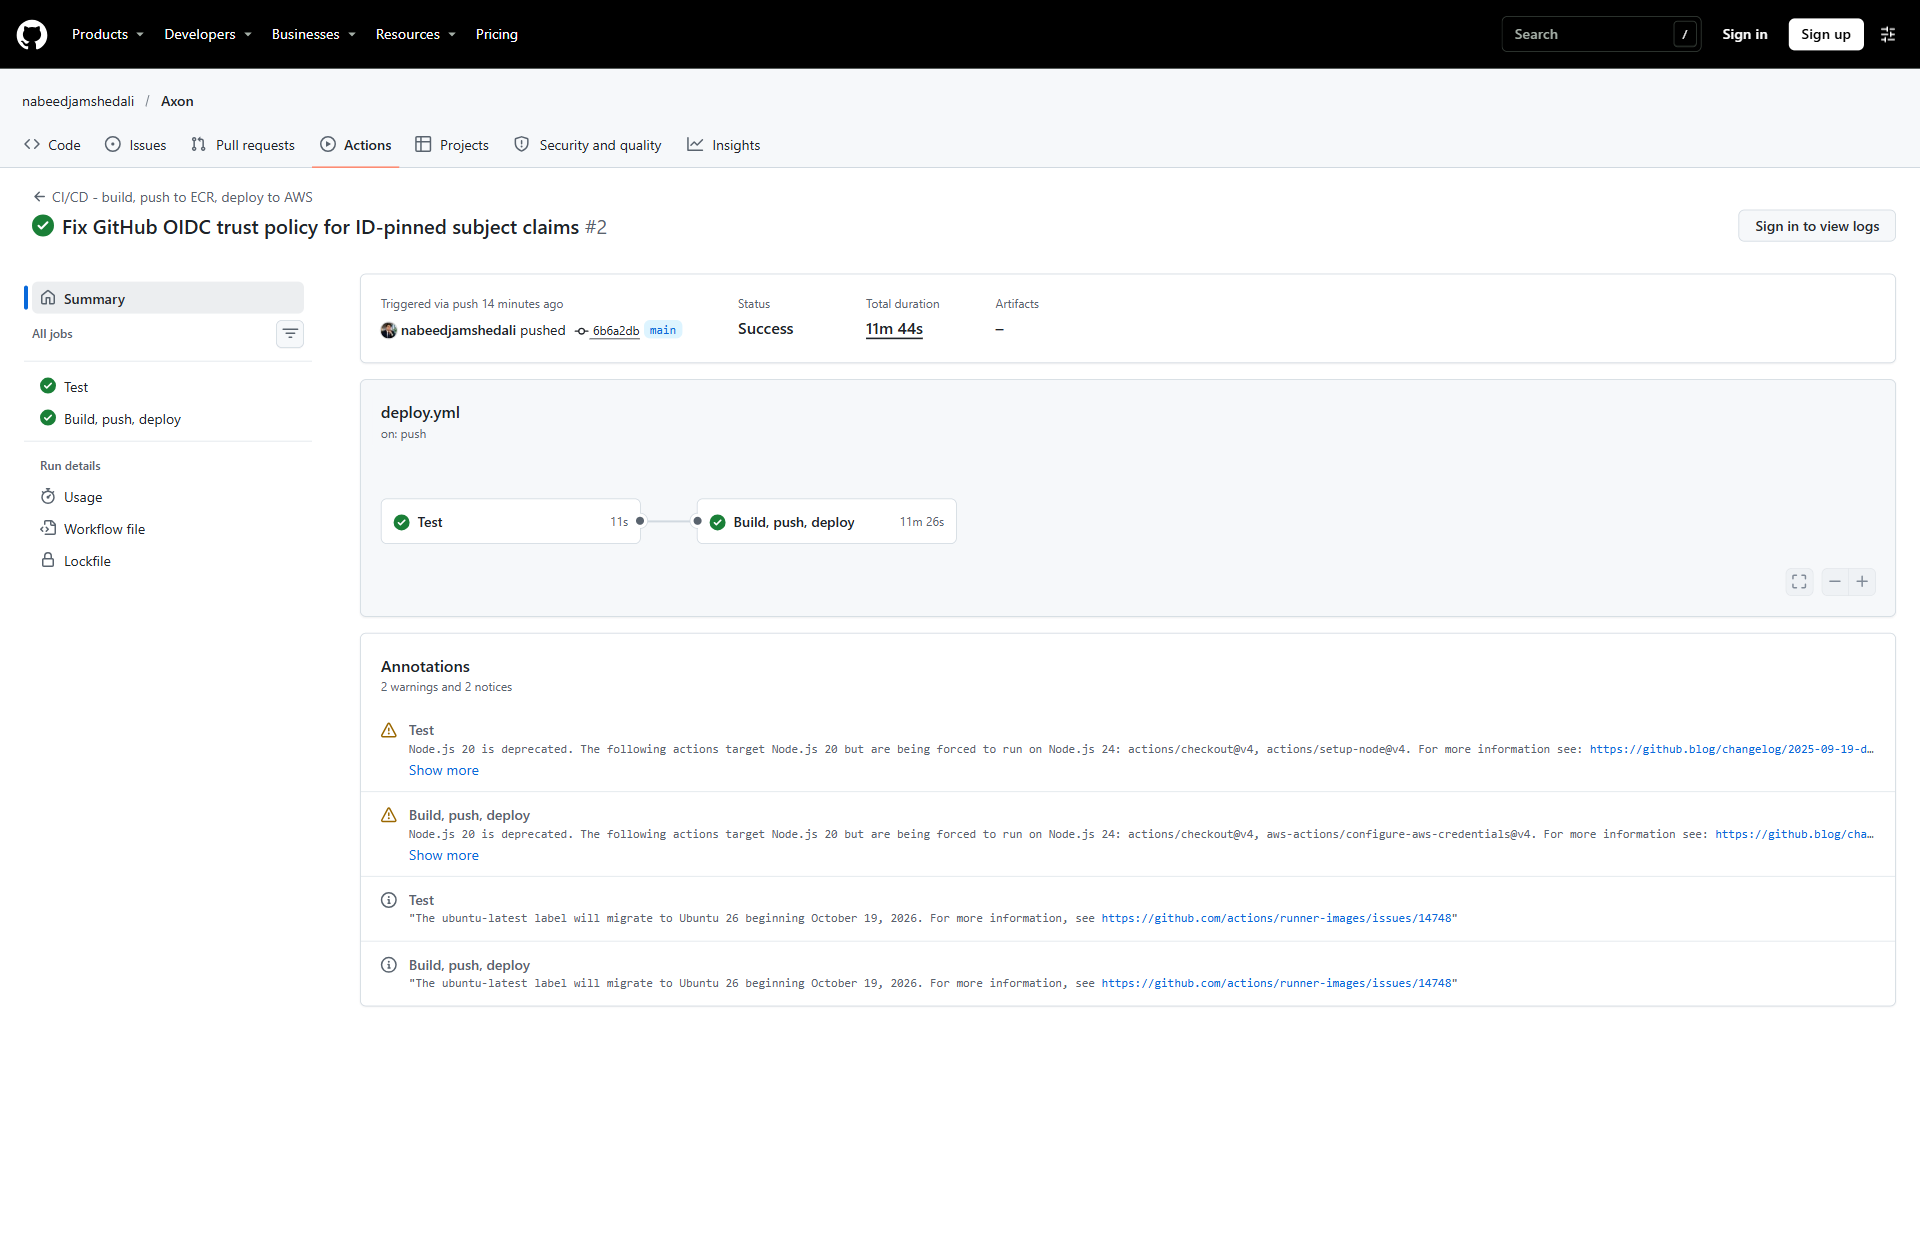
\includegraphics[width=\textwidth]{images/23-github-actions-run.png}\caption{Successful GitHub Actions run: Test and Build, push, deploy.}\end{figure}
\section*{Running application}
\begin{figure}[H]\centering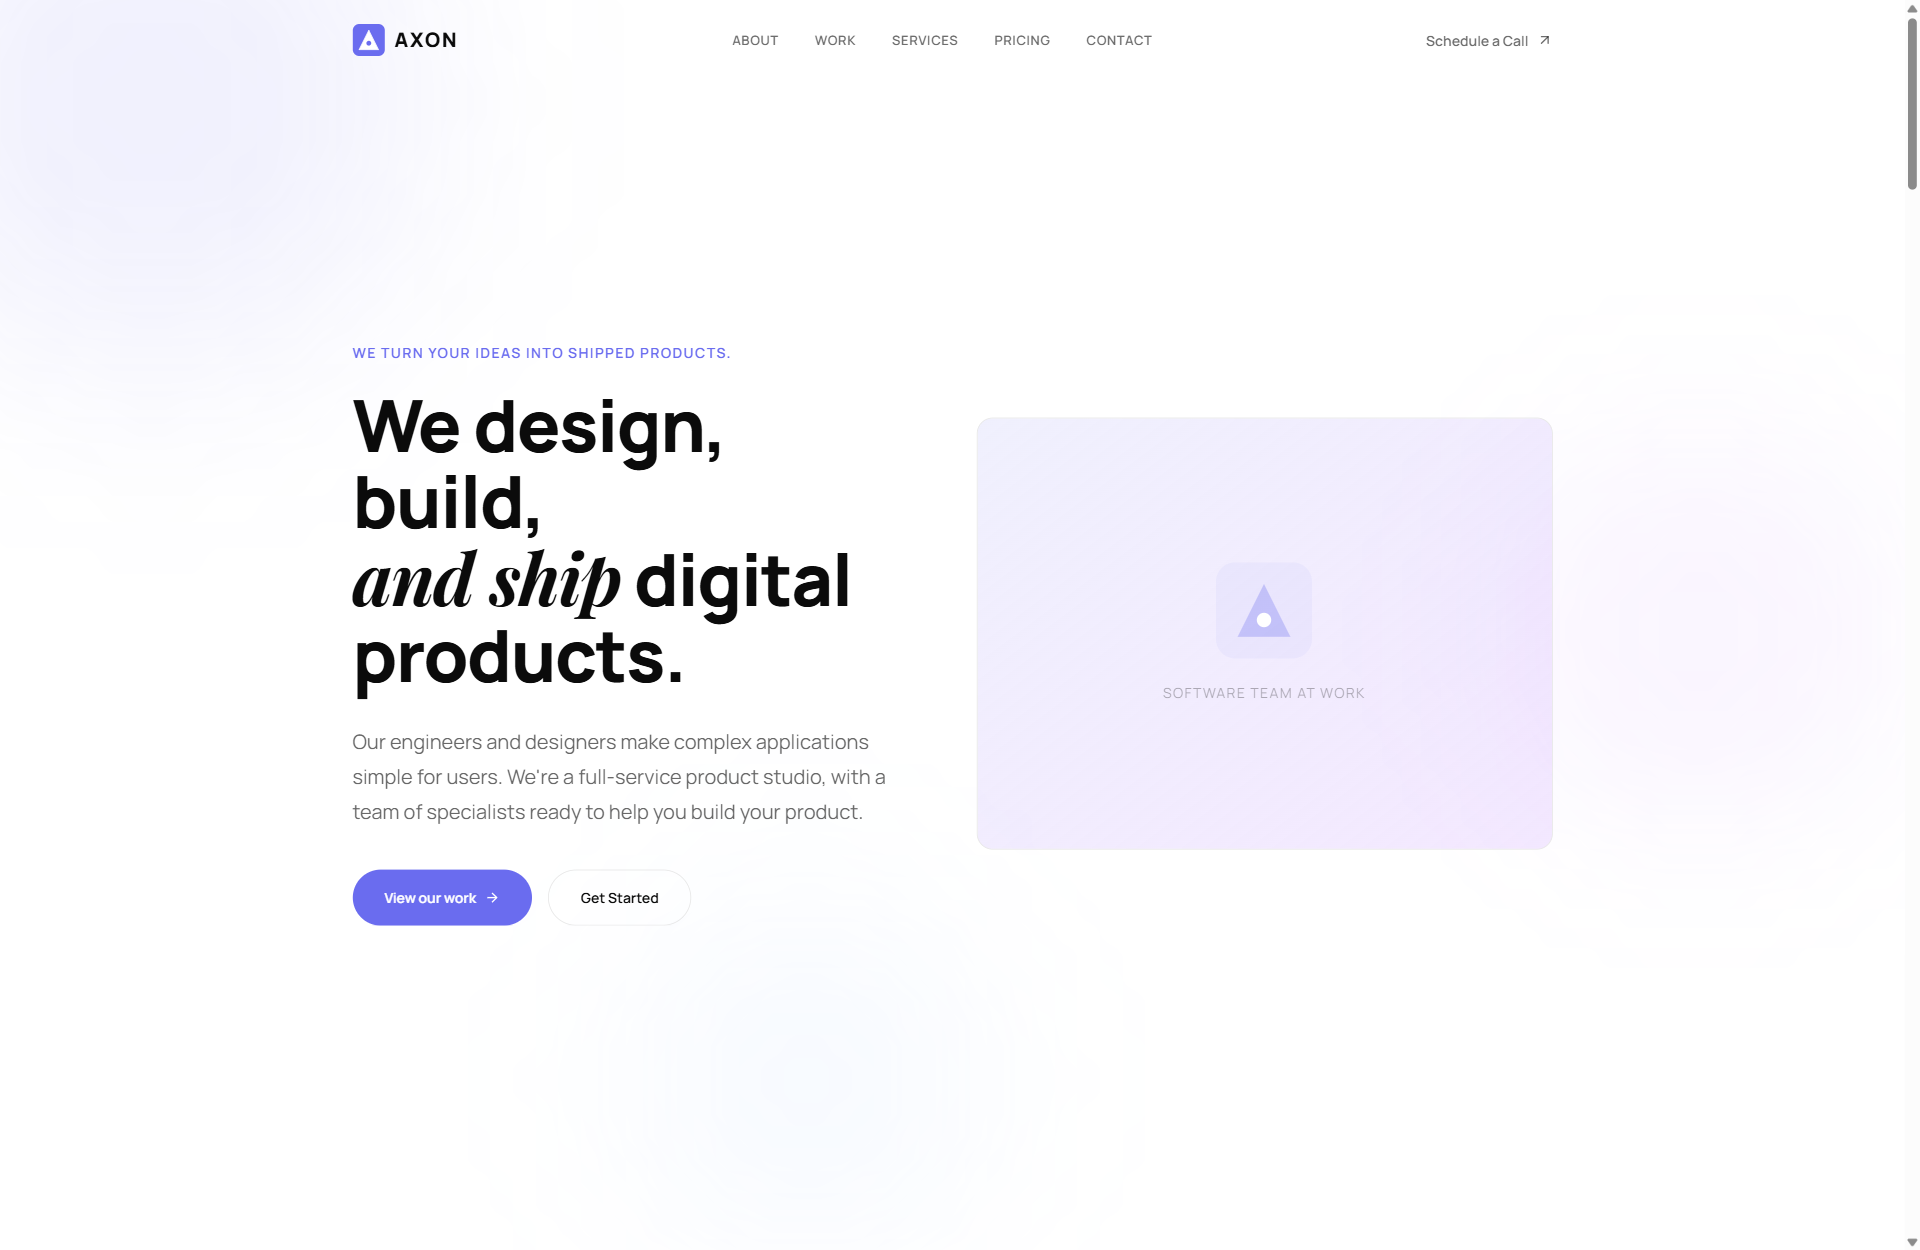
\includegraphics[width=\textwidth]{images/21-app-home.png}\caption{Application served through the public ALB.}\end{figure}
\begin{figure}[H]\centering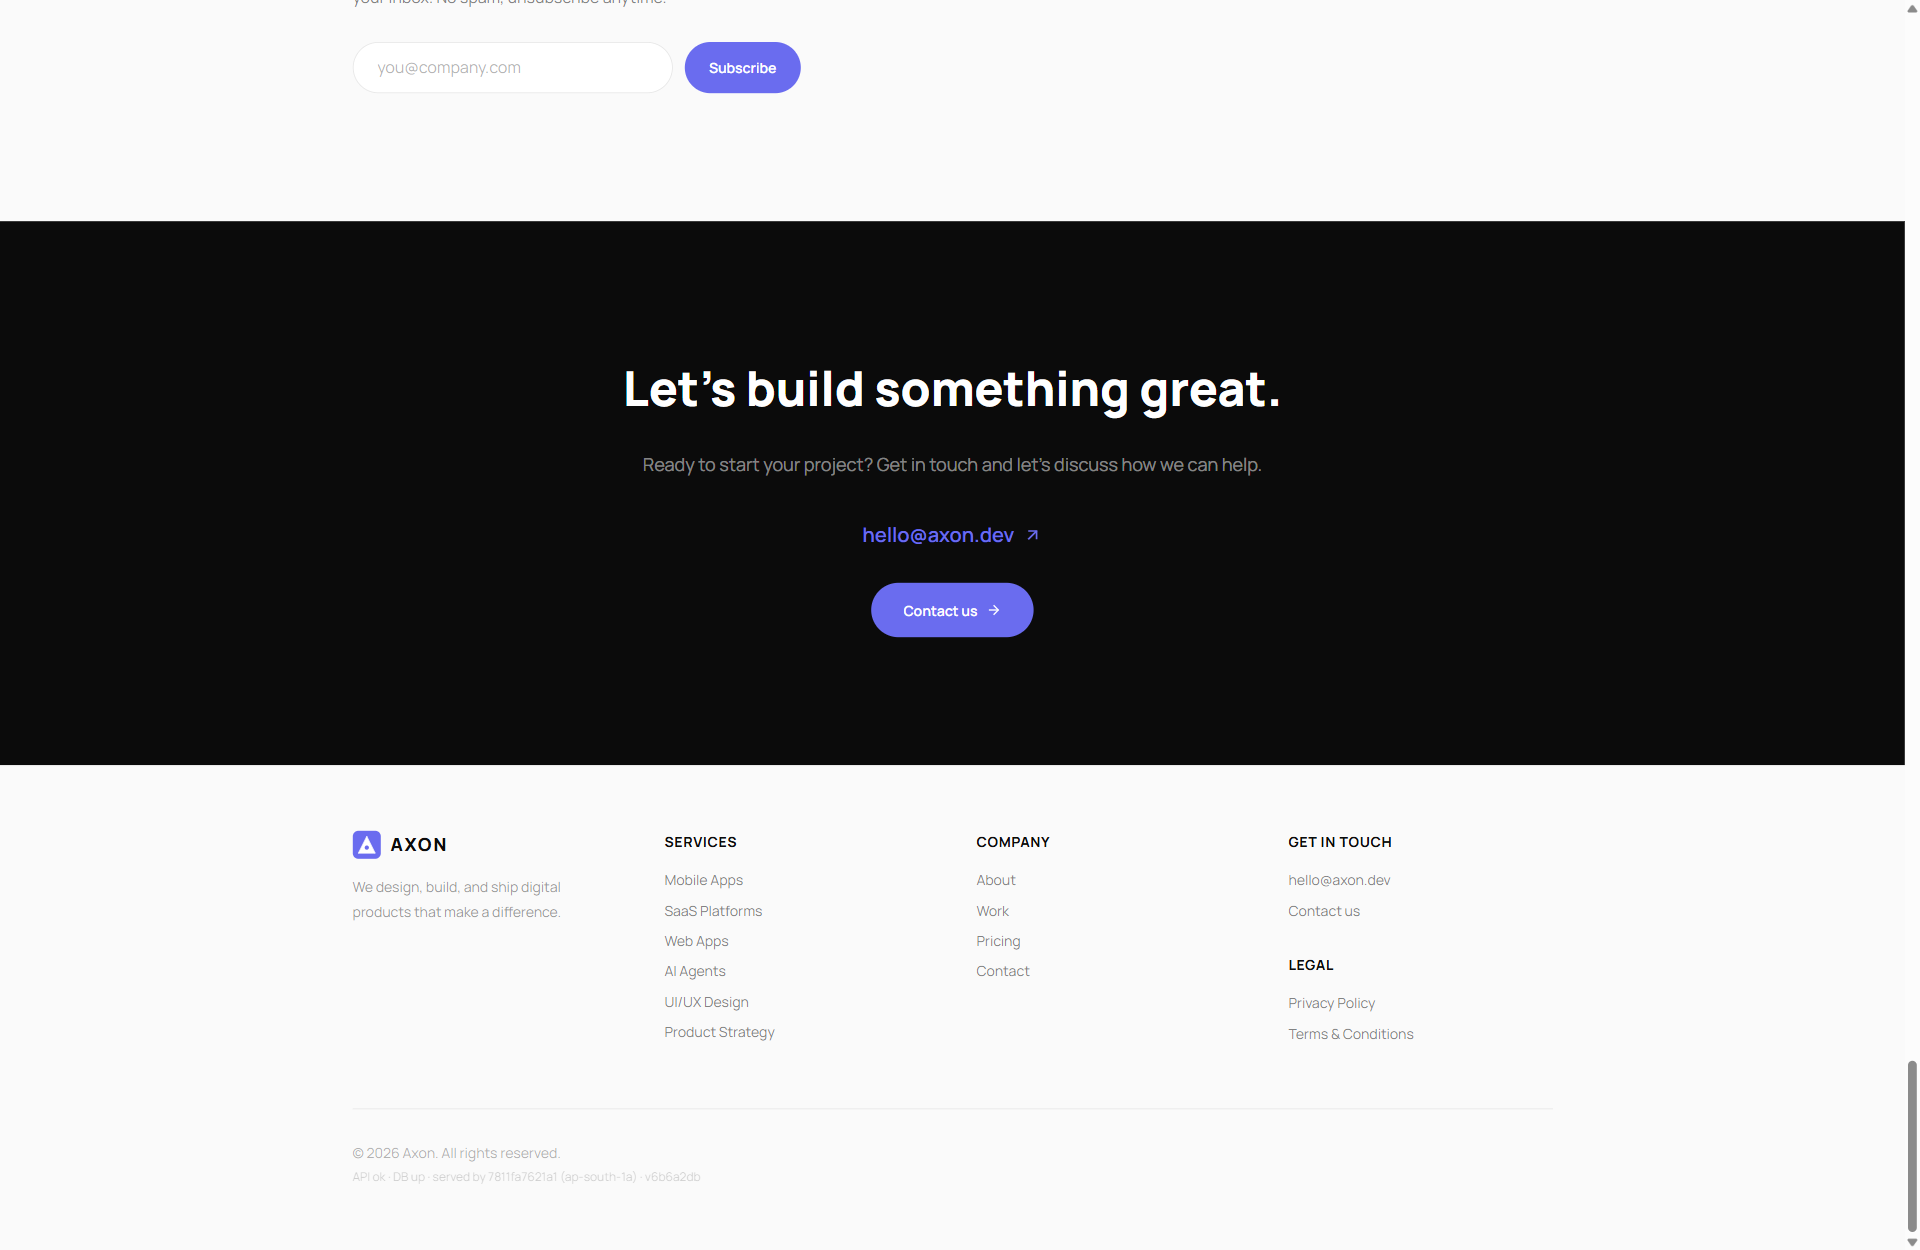
\includegraphics[width=\textwidth]{images/22-app-footer-status.png}\caption{Footer status line: API ok, DB up, serving instance, AZ and deployed commit.}\end{figure}
\section*{Additional cloud-native enhancements}
\begin{figure}[H]\centering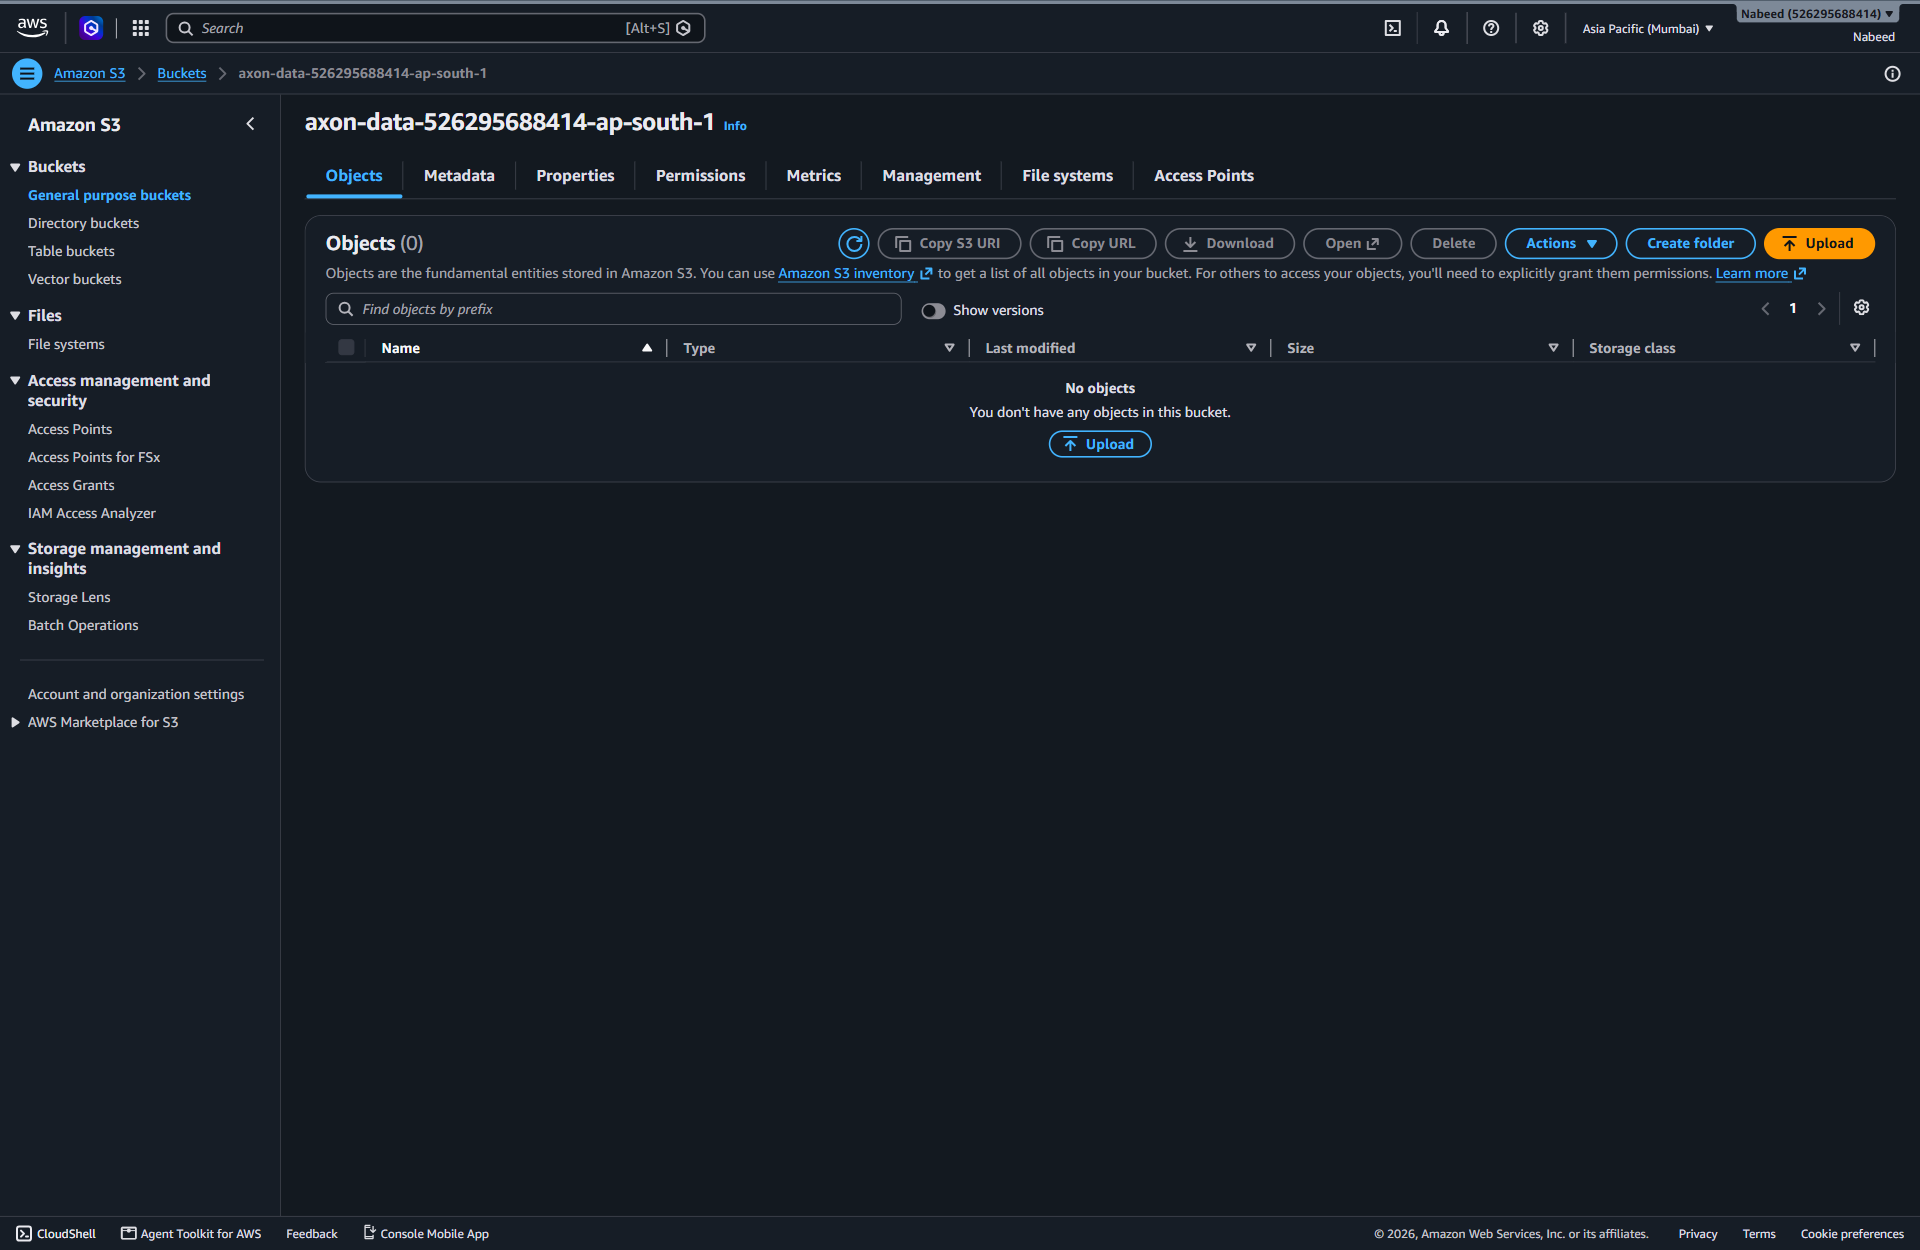
\includegraphics[width=\textwidth]{images/14-s3-bucket.png}\caption{S3 bucket for contact submissions (encrypted, private).}\end{figure}
\begin{figure}[H]\centering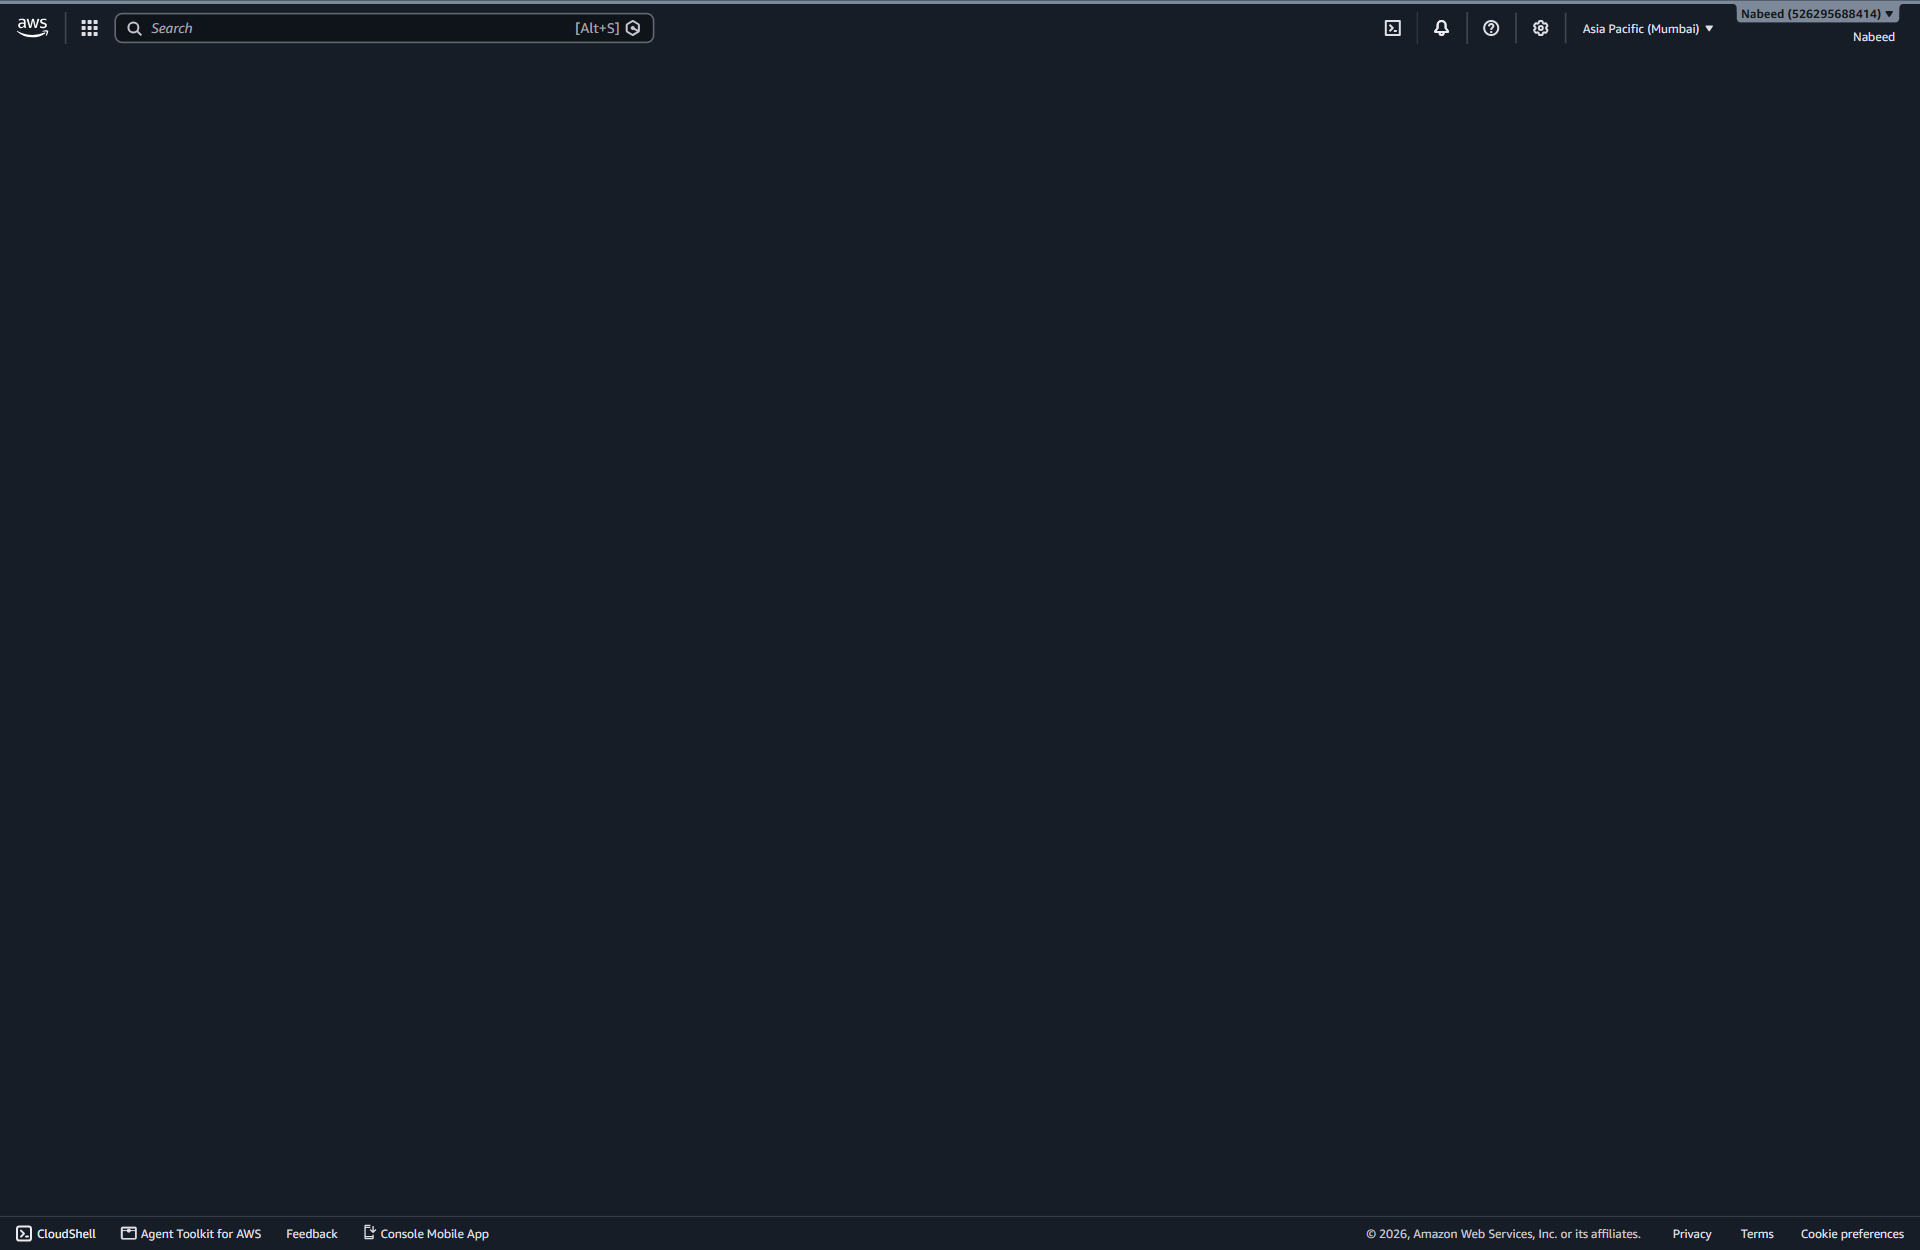
\includegraphics[width=\textwidth]{images/15-cloudwatch-dashboard.png}\caption{CloudWatch dashboard.}\end{figure}
\begin{figure}[H]\centering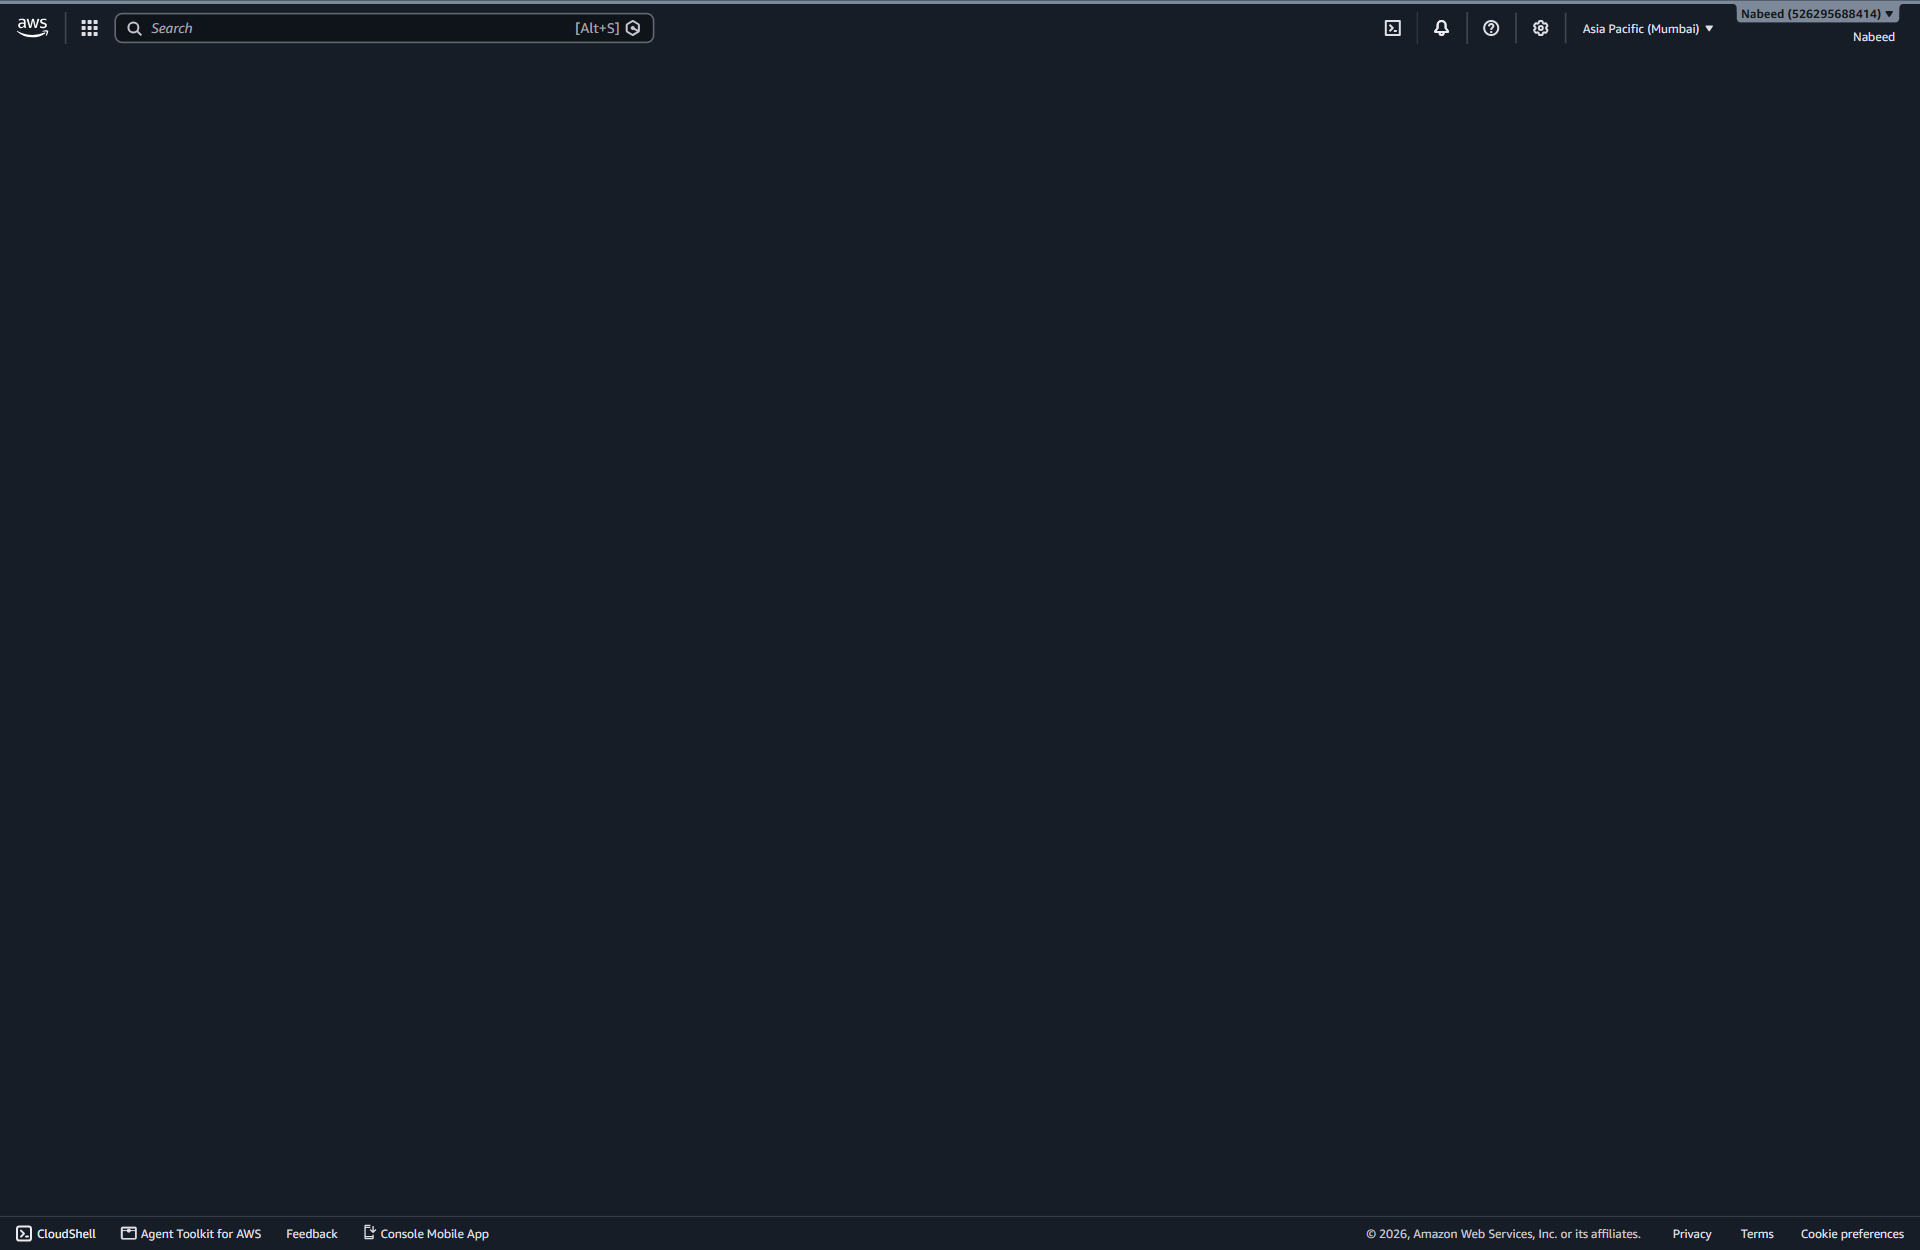
\includegraphics[width=\textwidth]{images/16-cloudwatch-logs.png}\caption{CloudWatch log groups for web and API containers.}\end{figure}
\end{document}
